\section{Introduction}
In this chapter, I aim to study the genetic toggle switch experimentally.  This chapter is organised as follows: In the first section I provide an overview of the circuit used and then outline the methods used for the experiments carried out. In the subsequent section I investigate the effect that the switch has on the growth rate of the bacteria. Then I examine the concentrations of the inducers and the time needed to flip the switch. 

\section{Circuit overview}

The toggle switch plasmid I used here was provided by ~\textcite{Litcofsky:2012gr}. All the switch components were contained in one plasmid, pKDL071. An overview of the plasmid is shown in Figure~\ref{fig:pKDL071map}A and the sequence given in Appendix (XXX). The circuit consists of two promoters, Ptrc2 and PLtetO-1~\autocite{Lutz:1997ti}. Ptrc2 is a constitutive promoter, repressible by LacI. PLtetO-1 is also a constitutive promoter, repressible by TetR, as shown in Figure~\ref{fig:pKDL071map}B. mCherry~\autocite{Shaner:2004vy} and \acrshort{gfp}~\autocite{SHIMOMURA:1962va} are fluorescent proteins, that were added under the control of the same promoters as the repressors, and thus reflect the levels of TetR and LacI in the system. The plasmid contains kanamycin antibiotic resistance and is high copy (ColE1 origin of replication).

This system is capable of two states, GFP high and mCherry high. When \acrshort{iptg} is added to the system, it represses the repression of TetR and mCherry and thus the cells end up in the mCherry high state. When \acrshort{atc} is added to the system, it represses the repression of LacI and GFP and thus the cells end up in the GFP high state. If no inducer is added to the system it will randomly go to one or the other. 


\begin{figure*}[tb]
	\begin{center}
		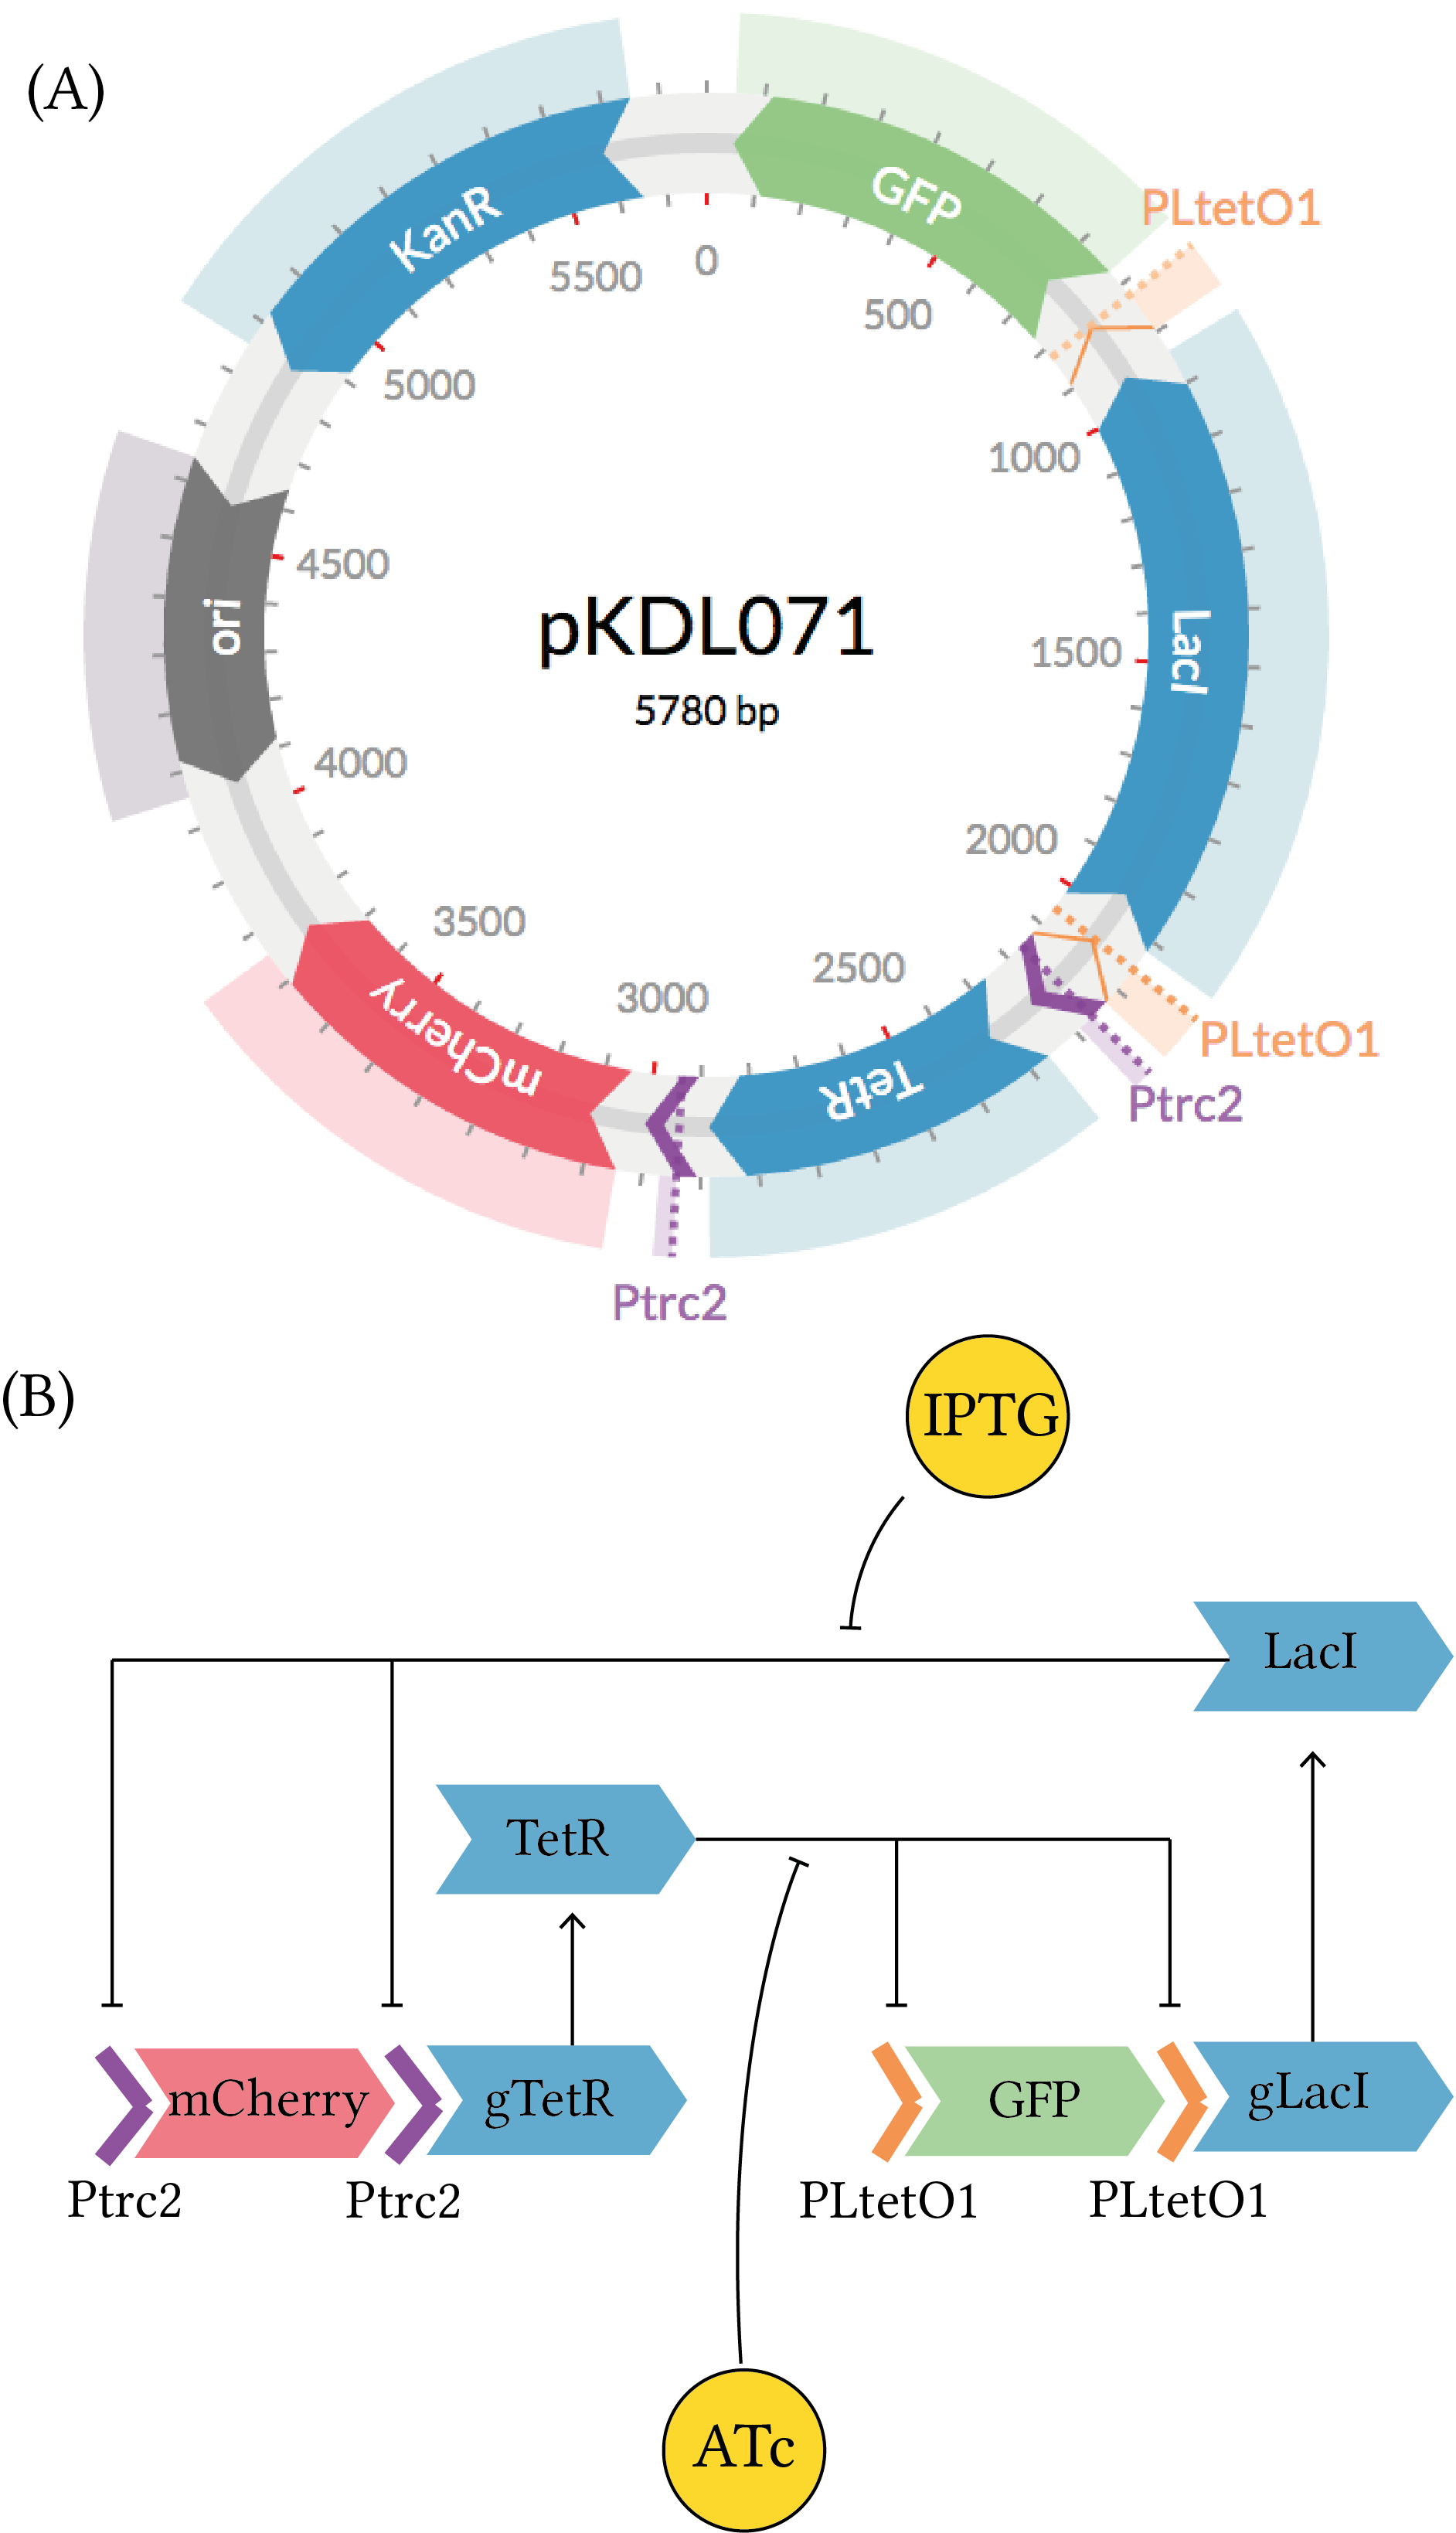
\includegraphics[scale=0.55]{chapterCharacterisation/images/pKDL071_overview.png}
	\caption[LoF caption]{\label{fig:pKDL071map}: The genetic toggle switch circuit used in this chapter. (A) The plasmid map of pKDL071, the plasmid containing the genetic toggle switch used in~\textcite{Litcofsky:2012gr} (B) The interactions between each element of the circuit.}
	\end{center}
\end{figure*}
\clearpage

\section{Methods}

The toggle switch plasmid was provided by the James J Collins lab in the form of a stab culture in \textit{E. coli} K-12 MG1655.

\subsection{\textit{Escherichia coli} culturing conditions}
\label{sec:overnigh_cult}

\acrfull{lb} was made by diluting \acrshort{lb} in deionized water to a concentration of \SI{25}{\gram\per\liter} and subsequently autoclaved. \acrshort{lb} agar plates were made by adding bacteriological agar to the above solution to a concentration of \SI{45}{\milli\gram\per\milli\liter} before autoclaving. The solution was then cooled down to \SI{55}{\celsius} using a water bath. If antibiotic was required it was added to the correct concentration to the cooled solution. The solution was then aliquoted to plates and left to solidify in room temperature. The plates were stored in the fridge for up to 1 month. 

Overnight cultures were made by picking a single colony from a static culture in an agar plate. Each colony was placed in \SI{15}{\milli\liter} Falcon tubes (Fisher Scientific, MA, U.S.A) with \SI{5}{\milli\liter} \acrshort{lb} with kanamycin antibiotic at a concentration of \SI{50}{\micro\gram\per\milli\liter}. The tubes were then screwed loosely and taped securely in order to allow for aeration. The falcon tubes were put in an incubator at \SI{37}{\celsius} with orbital shaking at \SI{200} rpm for 12-16 hours. 

\subsection{Inducers}

Anhydrotetracycline (ATc) solution was made by diluting \acrshort{atc} from Cayman Chemical Company in \SI{100}\% ethanol to a concentration of \SI{1}{\milli\gram\per\milli\liter}. \acrfull{iptg} solution was made by dissolving \acrshort{iptg} in deionized water to a concentration of \SI{1}{\molar}. The solution was sterilised by passing the solution through a \SI{0.22}{\micro\meter} syringe filter. Both inducers were stored in \SI{1}{\milli\liter} aliquots at \SI{-20}{\celsius}. 

\subsection{Glycerol stock preparation}
\label{sec:glycerol_stock}
To preserve the transformed cultures long term glycerol stocks were made. \SI{5}{\milli\liter} \acrshort{lb} and Kanamycin overnight cultures were made as described in Section~\ref{sec:overnigh_cult}. The cultures were kept on ice and \SI{70}\% glycerol was added to the cultures in a ratio of glycerol to culture of 1:7. These were aliquoted into cryovials and transferred to a \SI{-80}{\celsius} freezer for long-term storage.


\subsection{Revival}
For subsequent revival of the frozen cultures, a \SI{1.5}{\milli\liter} eppendorf tube was removed from the \SI{-80}{\celsius} freezer and put on ice. Small amount was streaked onto an agar plate containing \acrshort{lb} and kanamycin. The plates were stored in an incubator at \SI{37}{\celsius} overnight. Then the plates were sealed using parafilm and stored at \SI{4}{\celsius} for up to two weeks. 


\subsection{Plasmid construction}

I constructed two plasmids in order to used them for the flow cytometry experiments. The first plasmid, pSEVA281G contains the promoter PLtetO-1 and \acrshort{gfp} and the other, pSEVA281C, contains the promoter Ptrc2 and mCherry from PKDL071, shown in Figure~\ref{fig:psevas}. I used these two plasmids to determine the appropriate voltages for the lasers that excite \acrshort{gfp} and mCherry.

I constructed pSEVA281G by digesting pKDL071 and pSEVA281 using the protocol outlined in Section~\ref{sec:digest}. pSEVA281 is a plasmid backbone containing kanamycin resistance, a high copy origin of replication and a multiple cloning site. I isolated the digested fragments using gel purification (Section~\ref{sec:gel_electr}) and then ligated the isolated fragments (Section~\ref{sec:ligation}). I then transfected \textit{Escherichia coli} Dh5\textalpha{} with each plasmid (Section~\ref{sec:transfection}). pSEVA281C was constructed via \acrshort{pcr} cloning. I carried out a \acrshort{pcr} using the pKDL071 plasmid as a template \acrshort{dna} using the protocol outlined in Section~\ref{sec:pcr}. I chose the primers so that Ptrc2 and mCherry were copied and a Hind\RNum{3} restriction enzyme recognition sequence added to the fragment. The primers are listed in Appendix (XXX). I purified the amplified \acrshort{dna} using the Qiagen PCR cleanup kit (Qiagen, Crawley, U.K) and then carried out the rest of the cloning procedure as per plasmid pSEVA281G.

Following construction, I isolated each plasmid using the QIAprep Spin Miniprep Kit (Qiagen, Crawley, U.K). I determined plasmid concentration using the Thermo Scientific NanoDrop 1000 Spectrophotometer (Fisher Scientific, MA, U.S.A).

\begin{figure*}[t]
	\begin{center}
		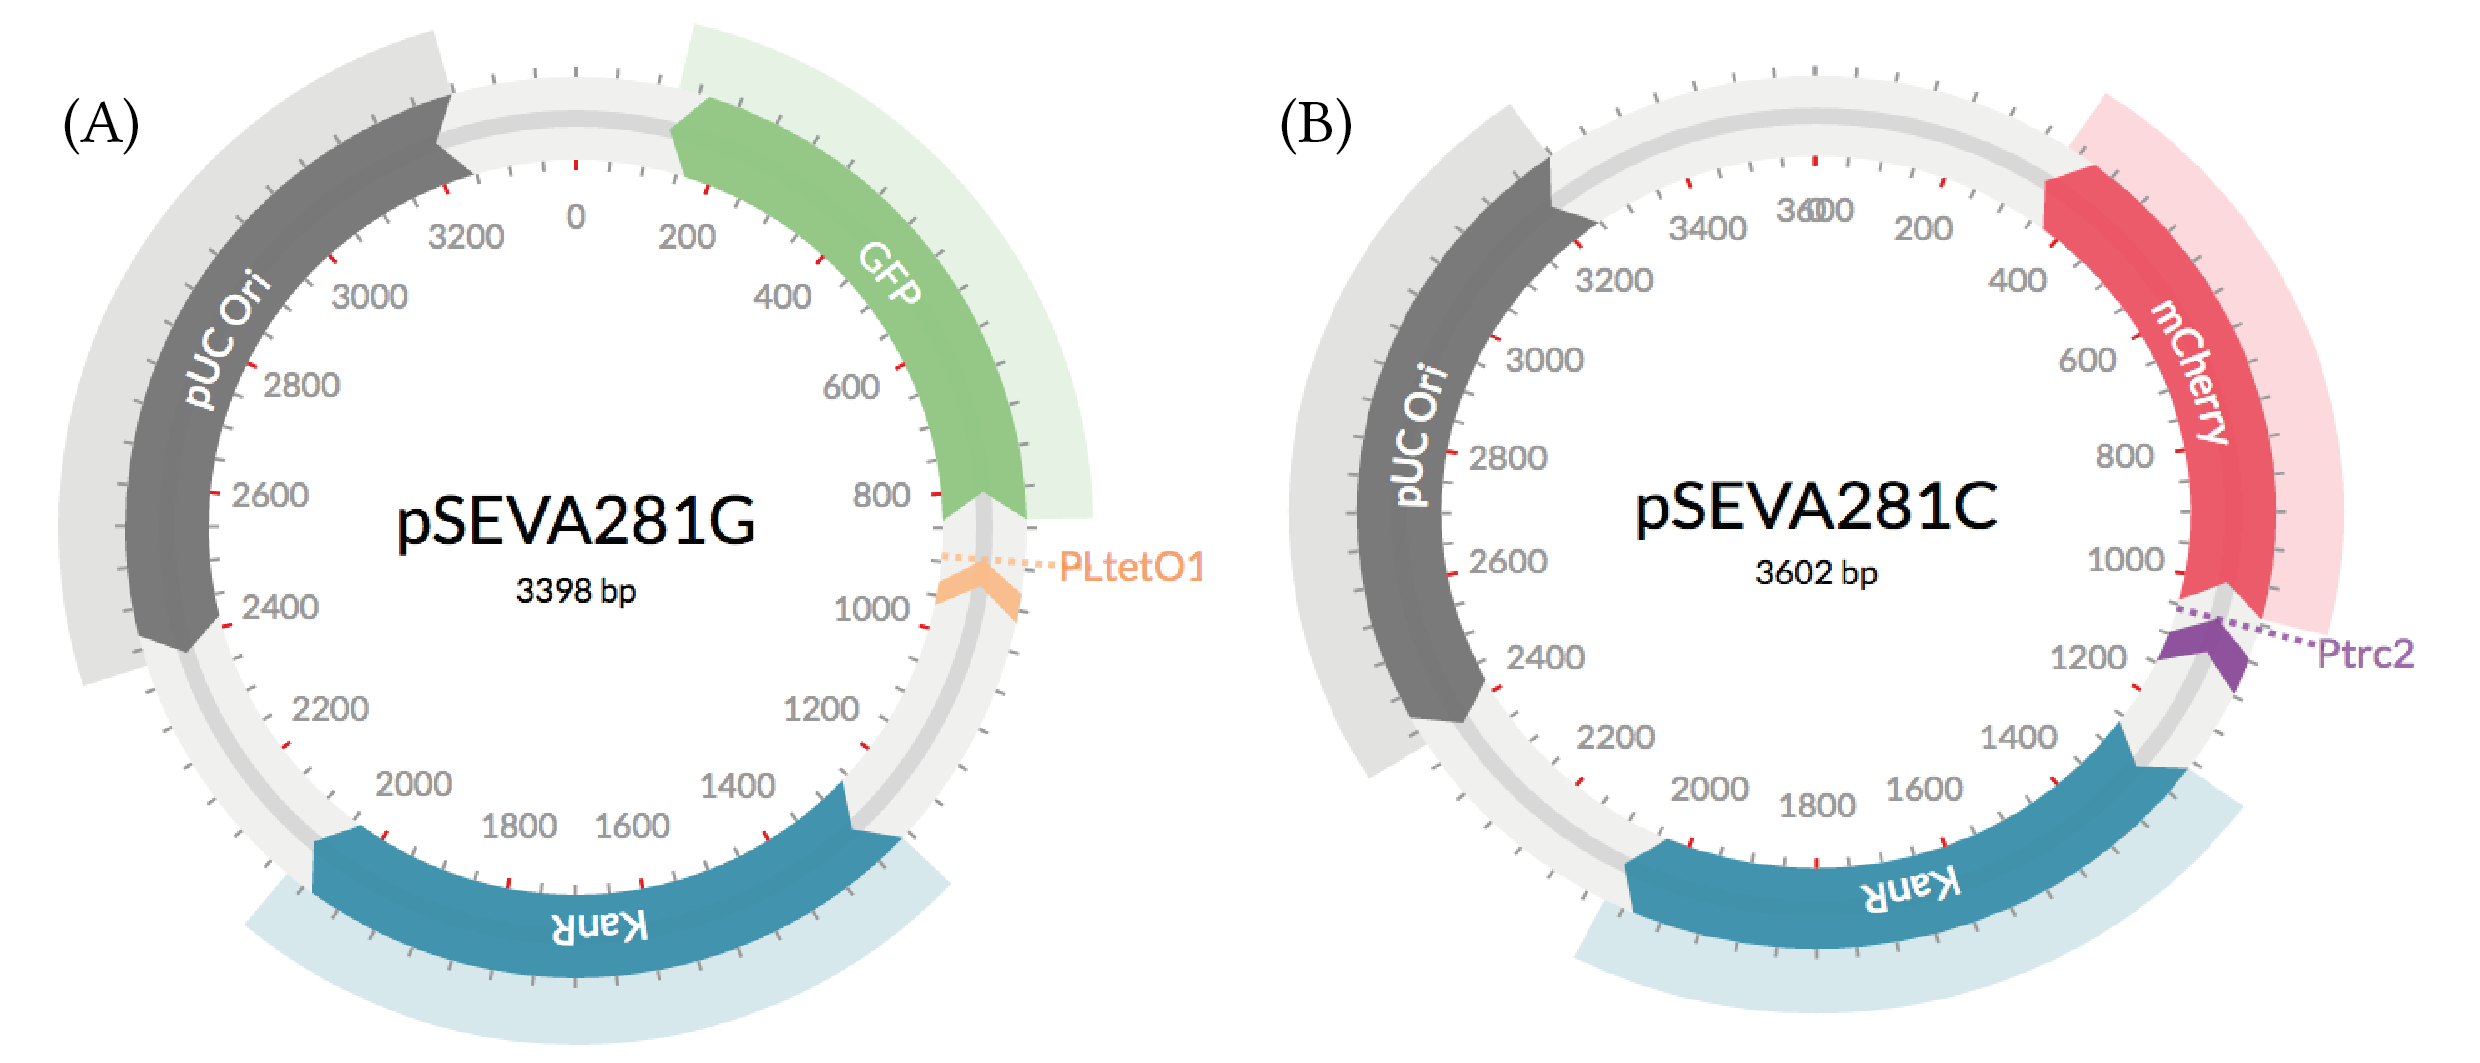
\includegraphics[width=\textwidth]{chapterCharacterisation/images/plasmids_constructed.png}
		\caption[LoF caption]{\label{fig:psevas}: The plasmids used to calibrate GFP and mCherry fluorescence. (A) pSEVA281G plasmid map (B) pSEVA281C plasmid map.  }
	\end{center}
\end{figure*}

\subsubsection{Polymerase Chain Reaction}
\label{sec:pcr}
In order to amplify DNA and add the restriction enzyme sites required, I carried out a \acrfull{pcr} reaction with mutagenic primers. A list of primers can be found in Appendix (XXX). I used the Q5\textsuperscript{\textregistered} DNA Polymerase (NEB, MA, U.S.A) with its associated buffer, \acrshort{dntp} and Q5\textsuperscript{\textregistered} enhancer, as specified in Table~\ref{tab:pcr_rec}. \acrshort{pcr} reactions were run in a T100\textsuperscript{TM} thermal cycler (Bio-Rad Laboratories, Inc., UK) as per the Q5\textsuperscript{\textregistered} recommendations, and as outlined in Tables~\ref{tab:pcr_rec} and ~\ref{tab:pcr_sched}.

\begin{table}[H]
\centering
\caption{\acrshort{pcr} recipe}
\label{tab:pcr_rec}
\begin{tabular}{@{}ccc@{}}
\toprule
Reagent           & Final concentration & \SI{50}{\micro\liter} reaction \\ \midrule
Q5\textsuperscript{\textregistered} buffer 5X      & 1X                  & \SI{10}{\micro\liter}          \\
\acrshort{dntp}             & \SI{200}{\milli\molar} each          & \SI{1}{\micro\liter}           \\
Forward primer    & \SI{0.5}{\micro\molar}               & \SI{2.5}{\micro\liter}         \\
Reverse primer    & \SI{0.5}{\micro\molar}               & \SI{2.5}{\micro\liter}         \\
Template DNA      & \SI{2}{\micro\gram}/\SI{50}{\micro\liter}                 & -             \\
Q5\textsuperscript{\textregistered} \acrshort{dna} polymerase & \SI{0.02}{\unit\per\micro\liter}            & \SI{0.5}{\micro\liter}         \\
Q5\textsuperscript{\textregistered} enhancer       & 1X                  & \SI{10}{\milli\liter}          \\
\ce{H2O}               & -                   & to \SI{50}{\micro\liter}       \\ \bottomrule
\end{tabular}
\end{table}


\begin{table}[H]
\centering
\caption{Thermocycling conditions}
\label{tab:pcr_sched}
\begin{tabular}{@{}cccc@{}}
\toprule
Step            & Cycles              & Temperature           & Time                 \\ \midrule
Initiation      & 1                   & \SI{98}{\celsius} & \SI{30}{\second} \\
Denaturation    & \multirow{3}{*}{30} & \SI{98}{\celsius} & \SI{10}{\second} \\
Annealing        &                     & \SI{72}{\celsius} & \SI{20}{\second} \\
Extension       &                     & \SI{72}{\celsius} & \SI{2}{\minute}  \\
Final extension & 1                   & \SI{72}{\celsius} & \SI{2}{\minute}  \\
Hold            & 1                   & \SI{4}{\celsius}  & \infty            \\ \bottomrule  
\end{tabular}
\end{table}

\subsubsection{Digestion}
\label{sec:digest}

All enzymes, buffers and \acrfull{bsa} were supplied by NEB. I carried out digestion controls by adding \ce{H2O} instead of \acrshort{dna} in the digestion reaction. Additionally, during agarose gel electrophoresis uncut plasmid was run alongside the digested plasmid in order to detect the difference. 

I set up \SI{2}{\micro\gram} digests by mixing the plasmid with \SI{0.5}{\micro\liter} of each restriction enzyme, \SI{3}{\micro\liter} 10x buffer and \SI{3}{\micro\liter} 10x \acrshort{bsa}. I added \ce{H2O} to make the reaction to \SI{20}{\micro\liter}. The recipe used is shown in Table~\ref{tab:digestion}. I placed the reactions in an incubator at \SI{37}{\celsius} for 4 hours. Finally, I analysed the solutions using agarose gel electrophoresis (Section~\ref{sec:gel_electr}).


\begin{table}[htbp]
\centering
\caption{Digestion recipe}
\label{tab:digestion}
\begin{tabular}{@{}cccc@{}}
\toprule
Reagent   & Volume  &  &  \\ \midrule
Pst\RNum{1}&                \SI{0.5}{\micro\liter}     &  &  \\
Hind\RNum{3} &                \SI{0.5}{\micro\liter}     &  &  \\
NEB Buffer 2.1        & \SI{2}{\micro\liter}       &  &  \\
BSA            & \SI{0.2}{\micro\liter}     &  &  \\
\acrshort{dna}              & \SI{1}{\micro\gram}       &  &  \\
\ce{H2O}           & to \SI{20}{\micro\liter} &  &  \\ \bottomrule
\end{tabular}
\end{table}


\subsubsection{Agarose gel electrophoresis}
\label{sec:gel_electr}
To make a 0.8\% agarose gel, I diluted \SI{0.4}{\gram} agarose in \SI{50}{\milli\liter} 1X TAE buffer. It was further dissolved by microwaving for 1-3 minutes. I left the solution to cool for 5 minutes and then added \SI{1.5}{\micro\liter} gel red. I prepared gel trays by putting the well comb in place and taping the ends shut. I then poured the solution into the prepared gel trays and left to solidify for 20-30 minutes at room temperature.

I carried out agarose gel electrophoresis by placing the poured gels into the gel tanks. I then flooded the tank with 1X TAE buffer. I prepared the \acrshort{dna} to be analysedI use by adding \SI{4}{\micro\liter} loading dye to \SI{20}{\micro\liter} sample. I also used a negative control with \ce{H2O} instead of sample. I prepared the \acrshort{dna} ladder of choice by adding \SI{1}{\micro\liter} \ce{H2O} and \SI{1}{\micro\liter} dye to \SI{2}{\micro\liter} ladder. I added each sample to a well by pipetting. The agarose gel was ran at \SI{90}{\volt} until the dye was 80\% of the way down the gel, approximately 1 hour.

To purify the fragments from the agarose gel, I placed the gel was in a UV box. Using a sterile razor blade, I cut out the desired fragment and placed in a clean eppendorf tube. I isolated the \acrshort{dna} from the gel using the QIAquick Gel Extraction Kit.

\subsubsection{Ligation}
\label{sec:ligation}
I used a ratio of 3:1 of insert to recipient plasmid, \SI{1}{\micro\liter} T4\textsuperscript{\textregistered}  DNA ligase (NEB, MA, U.S.A) and \SI{2}{\micro\liter} ligase buffer. I added \ce{H2O} to make the reaction up to \SI{20}{\micro\liter}. The controls I used for each ligation reaction, are shown in Table~\ref{tab:lig-contr}. Control 1 is used to detect competent cell viability, control 2 background due to uncut vector, control 3 contamination and control 4 vector re-circularization.  

I placed the ligation reactions at \SI{4}{\celsius} for 12 hours. I then placed the reactions at \SI{65}{\celsius} for 10 minutes to heat inactivate the T4 DNA ligase enzyme. I then carried out a transfection as per Section~\ref{sec:transfection}.

\begin{table}[htbp]
\centering
\caption{Ligation controls}
\label{tab:lig-contr}
\begin{tabular}{@{}ccccc@{}}
\toprule
       & Control 1 & Control 2 & Control 3 & Control 4 \\ \midrule
Vector &  Uncut    & \cmark    & \cmark    & \xmark    \\
Insert &  \xmark    & \xmark    & \xmark    & \cmark    \\
Buffer &  \cmark    & \cmark    & \cmark    & \cmark    \\
\ce{H2O}    & \cmark    & \cmark    & \cmark    & \cmark    \\
Ligase &  \xmark    & \xmark    & \cmark    & \cmark    \\ \bottomrule
\end{tabular}
\end{table}
\subsubsection{Transfection}
\label{sec:transfection}
I transfected thermocompetent \textit{E.coli} Dh5\textalpha with the constructed plasmids. I added each ligation reaction to \SI{50}{\micro\liter} of thawed competent cells. The cells were subsequently kept on ice for 30 minutes, then I placed them at a \SI{42}{\celsius} water bath for \SI{45}{\second}. I then placed the cells back on ice for 15 minutes. Then I added \SI{500}{\micro\liter} of Super Optimal broth with Catabolite repression (SOC) to each ligation and placed in a \SI{37}{\celsius} shaking incubator for 3 hours. I subsequently pipetted \SI{500}{\micro\liter} and \SI{50}{\micro\liter} of each ligation onto petri dishes with LB agar and the appropriate antibiotic. The plates were incubated at \SI{37}{\celsius} for 12-16 hours. I used two controls for the transfection protocol, a positive control with no antibiotic in the LB agar and non-transfected cells and a negative control of non-transfected cells and LB agar with antibiotic. These ensure that the cells are viable and not contaminated respectively. 

Finally, I counted the number of colonies on each plate. I selected individual colonies from each transfection and grew each separately in \SI{5}{\milli\liter} LB medium for 12-16 hours at \SI{37}{\celsius}, 200 rpm. I prepared glycerol stocks from each culture, as per Section~\ref{sec:glycerol_stock}.



\subsubsection{Colony \acrshort{pcr}}

In order to determine if the fragment was successfully inserted into the vector \acrshort{dna} plasmid, I carried out diagnostic colony \acrshort{pcr}. I designed primers that amplified the multiple cloning site of the vector \acrshort{dna} plasmid. These can be found in Appendix (XXX). I made a \acrshort{pcr} master mix for the number of colonies to be amplified, 32, with an added 10\% to account for pipetting error. I used GoTaq\textsuperscript{\textregistered} Flexi \acrshort{dna} polymerase (Promega Corp., WI, U.S.A.) with its associated buffer, \acrshort{dntp} and \ce{MgCl2}and \ce{H2O}. The recipe for the master mix is shown in Table~\ref{tab:pcr_mastex_mix}.

\begin{table}[htbp]
\centering
\caption{Colony \acrshort{pcr} master mix recipe}
\label{tab:pcr_mastex_mix}
\begin{tabular}{@{}ccc@{}}
\toprule
Reagent           & Final concentration & Master mix \\ \midrule
GoTaq\textsuperscript{\textregistered} green Flexi buffer      & 1X                  & \SI{141}{\micro\liter}          \\
\acrshort{dntp}             & \SI{200}{\milli\molar} each          & \SI{14.1}{\micro\liter}           \\
Forward primer    & \SI{0.5}{\micro\molar}               & \SI{1.4}{\micro\liter}         \\
Reverse primer    & \SI{0.5}{\micro\molar}               & \SI{1.4}{\micro\liter}         \\
GoTaq\textsuperscript{\textregistered} Flexi polymerase & \SI{0.02}{\unit\per\micro\liter}            & \SI{3.5}{\micro\liter}         \\
\ce{MgCl2}       & 1X                  & \SI{42.2}{\micro\liter}          \\
\ce{H2O}               &     -               & \SI{465}{\micro\liter}       \\ \bottomrule
\end{tabular}
\end{table}

I then added \SI{19}{\micro\liter} from the master mix to each \acrshort{pcr} tube. I lifted each of the colonies from the transformation from the agar plate using a \SI{20}{\micro\liter} pipette tip and added it to a \acrshort{pcr} mix by mixing. I subsequently used the pipette tip to make a scratch into a clean agar plate, and labelled it. I then carried out a \acrshort{pcr} according to GoTaq\textsuperscript{\textregistered} Flexi polymerase recommendations, and as shown in Table~\ref{tab:pcr_sched_col}.

\begin{table}[H]
\centering
\caption{Thermocycling conditions for colony \acrshort{pcr}}
\label{tab:pcr_sched_col}
\begin{tabular}{@{}cccc@{}}
\toprule
Step            & Cycles              & Temperature           & Time                 \\ \midrule
Cell lysis      & 1                   & \SI{95}{\celsius} & \SI{10} minutes \\

Denaturation    & \multirow{3}{*}{35} & \SI{95}{\celsius} & \SI{30}{\second} \\
Annealing        &                     & \SI{50}{\celsius} & \SI{1} minute \\
Extension       &                     & \SI{72}{\celsius} & \SI{1}{\minute}  \\

Final extension & 1                   & \SI{72}{\celsius} & \SI{5}{\minute}  \\
Hold            & 1                   & \SI{4}{\celsius}  & \infty            \\ \bottomrule  
\end{tabular}
\end{table}

Finally I carried out a diagnostic agarose gel electrophoresis as outlined in Section~\ref{sec:gel_electr}.

\subsubsection{Sequencing}
In order to confirm plasmid identity, all plasmids were sequenced using Source Bioscience, Cambridge UK. I submitted \SI{10}{\micro\liter} of each plasmid DNA at a minimum of \SI{100}{\nano\gram\per\micro\liter} as per the requirements. I submitted primer sequences that were manufactured by Source Bioscience. Primers can be found in Appendix (XXX). 

\subsection{Growth rate measurement}
\label{sec:growth_meth}
I carried out a plate reader analysis in order to measure the growth of \textit{E.coli} over time. I made overnight cultures using the method shown in Section~\ref{sec:overnigh_cult}. I then diluted the overnight cultures by a 1:1000 ratio into a \SI{5}{\milli\liter} \acrshort{lb} + kanamycin solution. The diluted cultures were grown at \SI{37}{\celsius} with shaking at 200rpm for 1 hour. I then further diluted these cultures by a 1:100 ratio. I transferred \SI{200}{\ul} aliquots of the dilutions to a clear bottom, black-walled 96-well plate. I also added wells with only LB and kanamycin in order to be used as blanks. I then sealed the plate using a gas permeable membrane and placed it in BMG FLUOstat OPTIMA plate reader to measure absorbance. I set the plate reader to a constant \SI{37}{\celsius}, with 30 seconds orbital shaking at \SI{150}rpm and \SI{4}{\milli\metre} shaking width every ten minutes. Absorbance was measured at \SI{540}{\nano\meter}. Data was exported as a CSV file and analysed using Python. 

\subsection{Flow cytometry}
I carried out flow cytometry experiments in order to get fluorescent levels in single cells. Flow cytometry allows us to gather this information for thousands of single cells. Flow cytometry data was exported as FCS files and analysed using the R bioconductor package. 

\subsubsection{Concentration assays}
\label{sec:flo_conc}
I carried out concentration assays to determine the concentration of each inducer (\acrshort{atc} and \acrshort{iptg}) at which the switch flips.  I prepared separate overnight cultures as per Section~\ref{sec:overnigh_cult} with added \acrshort{iptg} at a concentration of \SI{1}{\milli\molar} or added \acrshort{atc} at a concentration of \SI{100}{\nano\gram\per\milli\liter}~\autocite{Litcofsky:2012gr}. I then diluted the cultures by 1:1000 into fresh \acrshort{lb} medium with varying concentrations of the opposite inducer than what the cells were grown in overnight. The concentrations used are shown in Table~\ref{tab:flow_conc}. For each concentration I made three replicates cultures.


\begin{table}[htbp]
\centering
\caption{Concentrations used for flow cytometry assay}
\label{tab:flow_conc}
\begin{tabular}{@{}cc@{}}
\toprule
\acrshort{atc} (ng/ml)  & \acrshort{iptg} (M) \\ \midrule
0.05 & 1e-7 \\
0.06 & 6e-7 \\
0.07 & 1e-6 \\
0.08 & 6e-6 \\
0.09 & 1e-5 \\
0.1  & 1e-3 \\
1.0  & 0.1  \\ \bottomrule
\end{tabular}
\end{table}

I placed the cultures in an incubator at \SI{37}{\celsius}, 200rpm for 5 hours. I then placed the cultures in a centrifuge and spun at 13,000rpm for 5 minutes. I discarded the supernatant and replaced it with \SI{1}{\milli\liter} PBS solution. I used the The BD LSRFortessa\textsuperscript{TM} cell analyzer (Becton, Dickinson and Company) at the St. Mary's Flow Cytometry Core Facility at Imperial College London  for flow cytometry analysis. \acrshort{gfp} was excited using the \SI{488}{\nano\meter} laser and detected using the 533/30 filter. mCherry was excited using the \SI{561}{\nano\meter} laser and detected using the 620/10 filter. Data was obtained at n=10000 events per experiment. 

\subsubsection{Time course assays}
\label{sec:flo_time}
I carried out time course assays to measure the time it takes for the switch to flip to each side. I prepared separate overnight cultures of pKDL071 as per Section~\ref{sec:overnigh_cult} with added \acrshort{iptg} at a concentration of \SI{1}{\milli\molar} or added \acrshort{atc} at a concentration of \SI{100}{\nano\gram\per\milli\liter}~\autocite{Litcofsky:2012gr}. I also made overnight cultures of pSEVA281G and pSEVA281C. I then diluted the cultures by a ratio of 1:1000 into fresh LB medium. I made separate cultures for each time point, in triplicates. For cultures grown overnight in \acrshort{iptg}, I added \acrshort{atc} at a concentration of \SI{100}{\nano\gram\per\milli\liter} and for cultures grown overnight in \acrshort{atc}, I added \acrshort{iptg} at a concentration of \SI{1}{\milli\molar}. All cultures were placed at \SI{37}{\celsius}, 200rpm incubator. At 30 minutes, 1 hour and then every hour up to 6 hours I carried out flow cytometry to the corresponding cultures. I removed three replicates for each induction from the incubator and placed them in a centrifuge at 13,000rpm for 10 minutes. I discarded the supernatant and replaced it with \SI{1}{\milli\liter} PBS solution. I then analysed these cultures in an Attune\textsuperscript{TM} NxT Flow Cytometer (Thermo Fisher Scientific) at University College London. \acrshort{gfp} was excited using the \SI{488}{\nano\meter} laser and detected using the 533/30 filter. mCherry was excited using the \SI{561}{\nano\meter} laser and detected using the 620/10 filter. Data was obtained at n=10000 events per experiment. I used pSEVA281G and pSEVA281C cultures to set the laser voltages and pKDL071 cultures to detect the bacteria population.  

\clearpage
\section{Growth rate investigation}

I carried out a growth rate analysis to determine whether the \acrshort{atc} or \acrshort{iptg} added to pKDL071 or pSEVA281G \textit{E. coli} cultures affected the growth of the bacteria. Cultures were grown without any inducer overnight as described in Section~\ref{sec:growth_meth}. I ran assays for the cultures with and without added inducers. As can be seen in Figure~\ref{fig:growth_curve}, there is no difference between the conditions. The addition of either \acrshort{atc} or \acrshort{iptg} does not affect the growth rate of \textit{E. coli} K-12 MG1655. Additionally, \acrshort{atc} does not affect the growth rate of \textit{E. coli} Dh5\textalpha. Since the addition of \acrshort{atc} flips the switch to the GFP high state, and \acrshort{iptg} to the mCherry high state, we can also conclude that the growth rate of the chassis is not affected by which side of the switch is in the high state. The growth rate of \textit{E. coli} Dh5\textalpha was consistently lower than that of \textit{E. coli} K-12 MG1655.

\begin{figure*}[htbp]
	\begin{center}
		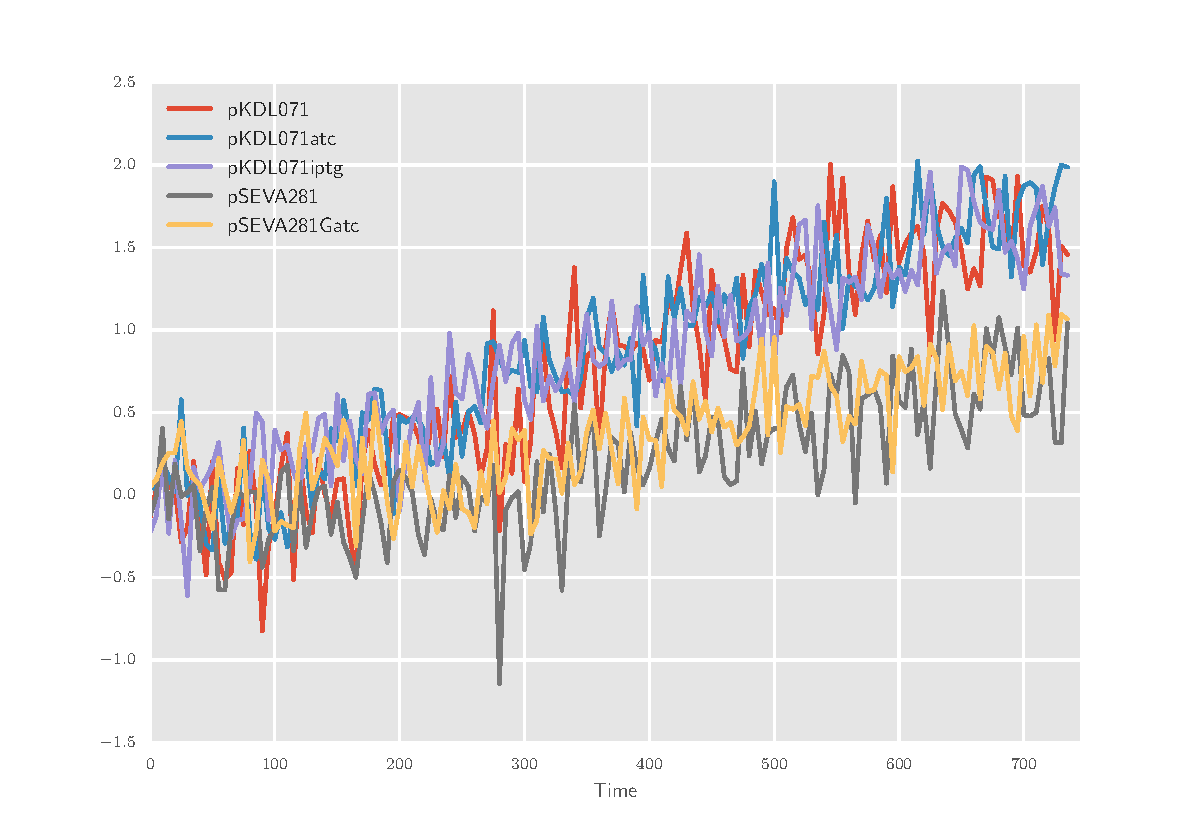
\includegraphics[scale=0.7]{chapterCharacterisation/images/growth_curves.pdf}
		\caption[LoF caption]{\label{fig:growth_curve}: Growth rate analysis of \textit{E. coli} K-12 MG1655 pKDL071 and \textit{E. coli} Dh5\textalpha pSEVA281G cultures with and without inducers. The inducers do not affect the growth of the bacteria. }
	\end{center}
\end{figure*}

\clearpage

\section{Toggle switch concentration assays}

Here I aim to identify the inducer concentration at which the pKDL071 toggle switch changes state. In order to do that I carry out a concentration assay using flow cytometry, as described in Section~\ref{sec:flo_conc}. As can be seen in Figure~\ref{fig:switch_concent2d1d}A, during \acrshort{atc} induction the switch flips to a GFP high state when \acrshort{atc} concentration is at \SI{0.09}{\nano\gram\per\milli\liter} or higher. We observe a bimodal distribution at concentrations \SI{0.07}{\nano\gram\per\milli\liter} and \SI{0.08}{\nano\gram\per\milli\liter}, which indicates that the switching has begun at these concentrations. Thats why part of the population has switched to the GFP high state but complete switching is not observed until the concentration of \acrshort{atc} is at \SI{0.09}{\nano\gram\per\milli\liter}. In the case of \acrshort{iptg} induction (Figure~\ref{fig:switch_concent2d1d}B) we find that the switch flips to the mCherry high state when the concentration of \acrshort{iptg} is higher or equal to 0.001M. A decrease in GFP fluorescence is also observed. We do not observe a bimodal distribution in this case. 

\begin{figure*}[htbp]
	\begin{center}
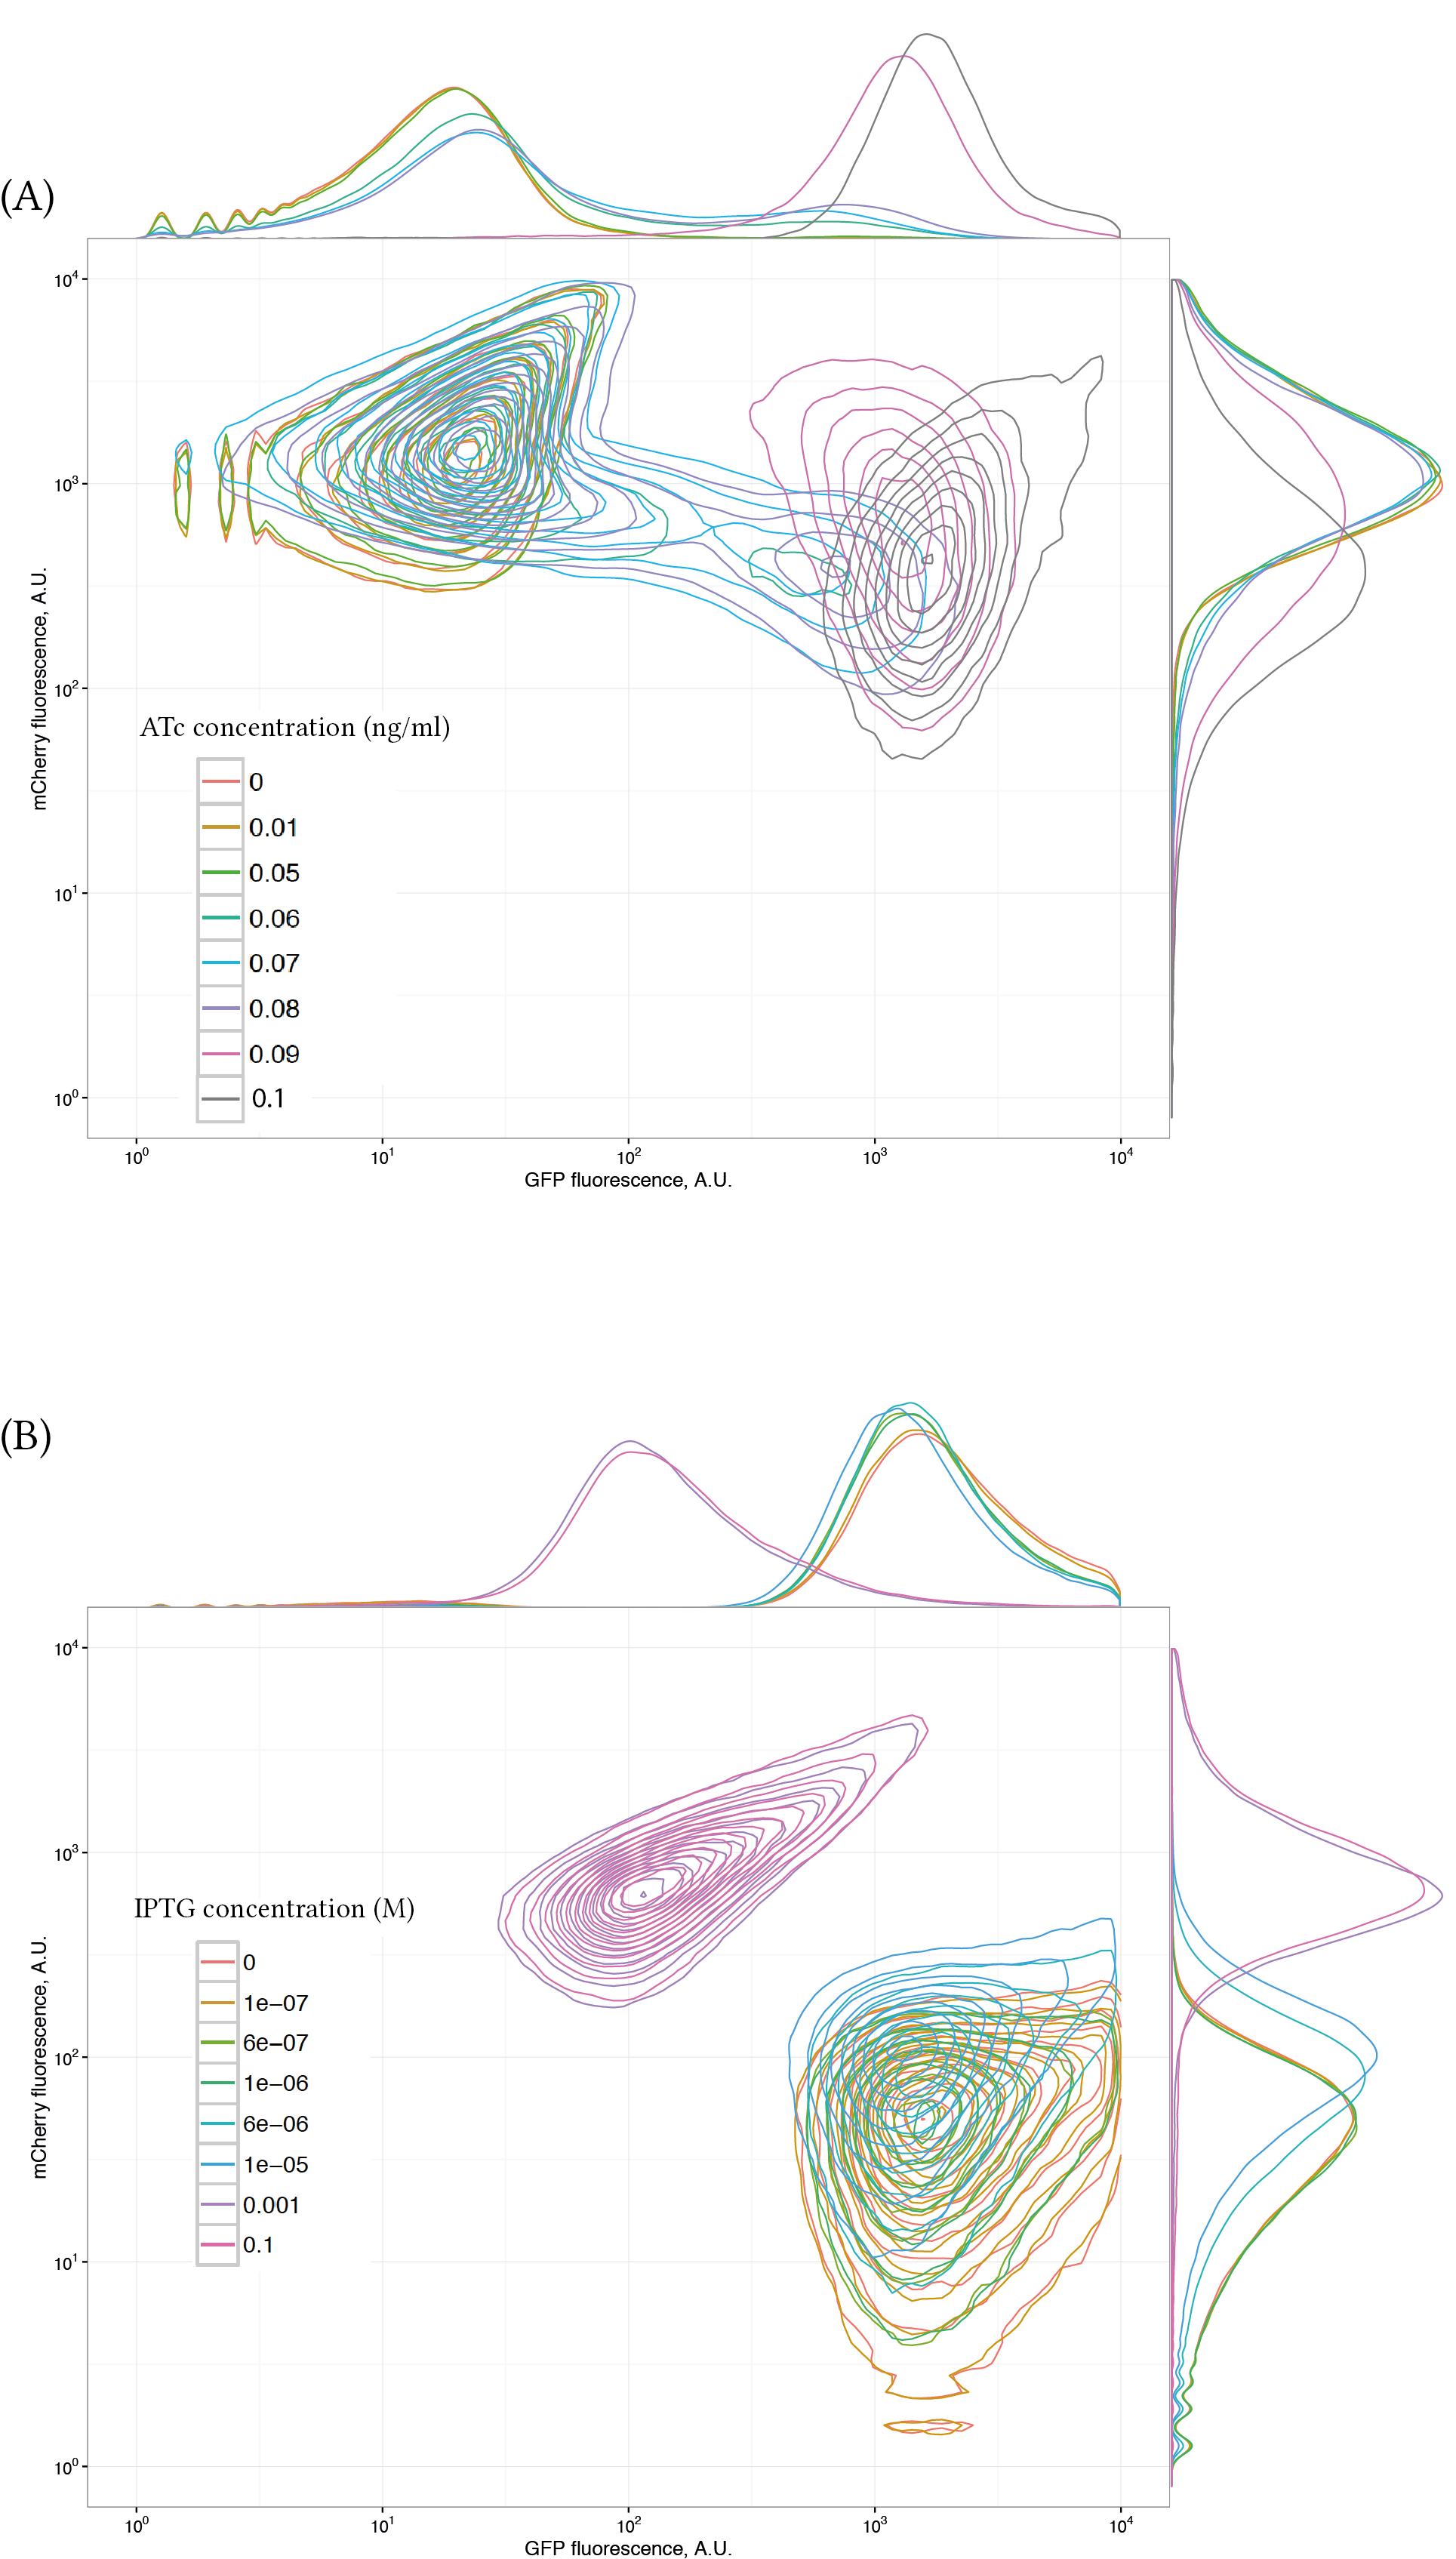
\includegraphics[scale=0.7]{chapterCharacterisation/images/pKDL071_concentrations_2d1d.png}
\caption[LoF caption]{\label{fig:switch_concent2d1d}: (A) \acrshort{atc} induction at various concentrations (B) \acrshort{iptg} induction at various concentrations. }
\end{center}
\end{figure*}
\clearpage

By taking into account the two induction curves of the switch turning to each high state, we can see the dynamic ranges of pKDL071 in \textit{E.coli}. We can see in Figure~\ref{fig:switch_concentrations_model} there is an approximately 100-fold change in fluorescent units during \acrshort{iptg} and \acrshort{atc} induction. 

 A Hill function was used to model the characterisation curves shown in Figure~\ref{fig:switch_concentrations_model}. The model used is the following:
 \begin{align}
 	F = Pmin + (Pmax - Pmin)\frac{\Big(\frac{[I]}{Kd}\Big)^n}{1+\Big(\frac{[I]}{Kd}\Big)^n},
 \end{align}
 
where F is the median fluorescent unit and [I] is the concentration of inducer. Pmin and Pmax are the minimum and maximum fluorescence respectively, and Kd and n are the dissociation constant, and Hill coefficient. I fit Hill function models using maximum likelihood estimation to the response curves. The values for parameters Pmin, Pmax, Kd, and n are 8, 1600, 0.1, 1.8 respectively for the \acrshort{atc} induction and 8, 700, 0.08, 2.5 for \acrshort{iptg} induction. 

\begin{figure*}[tb]
	\begin{center}
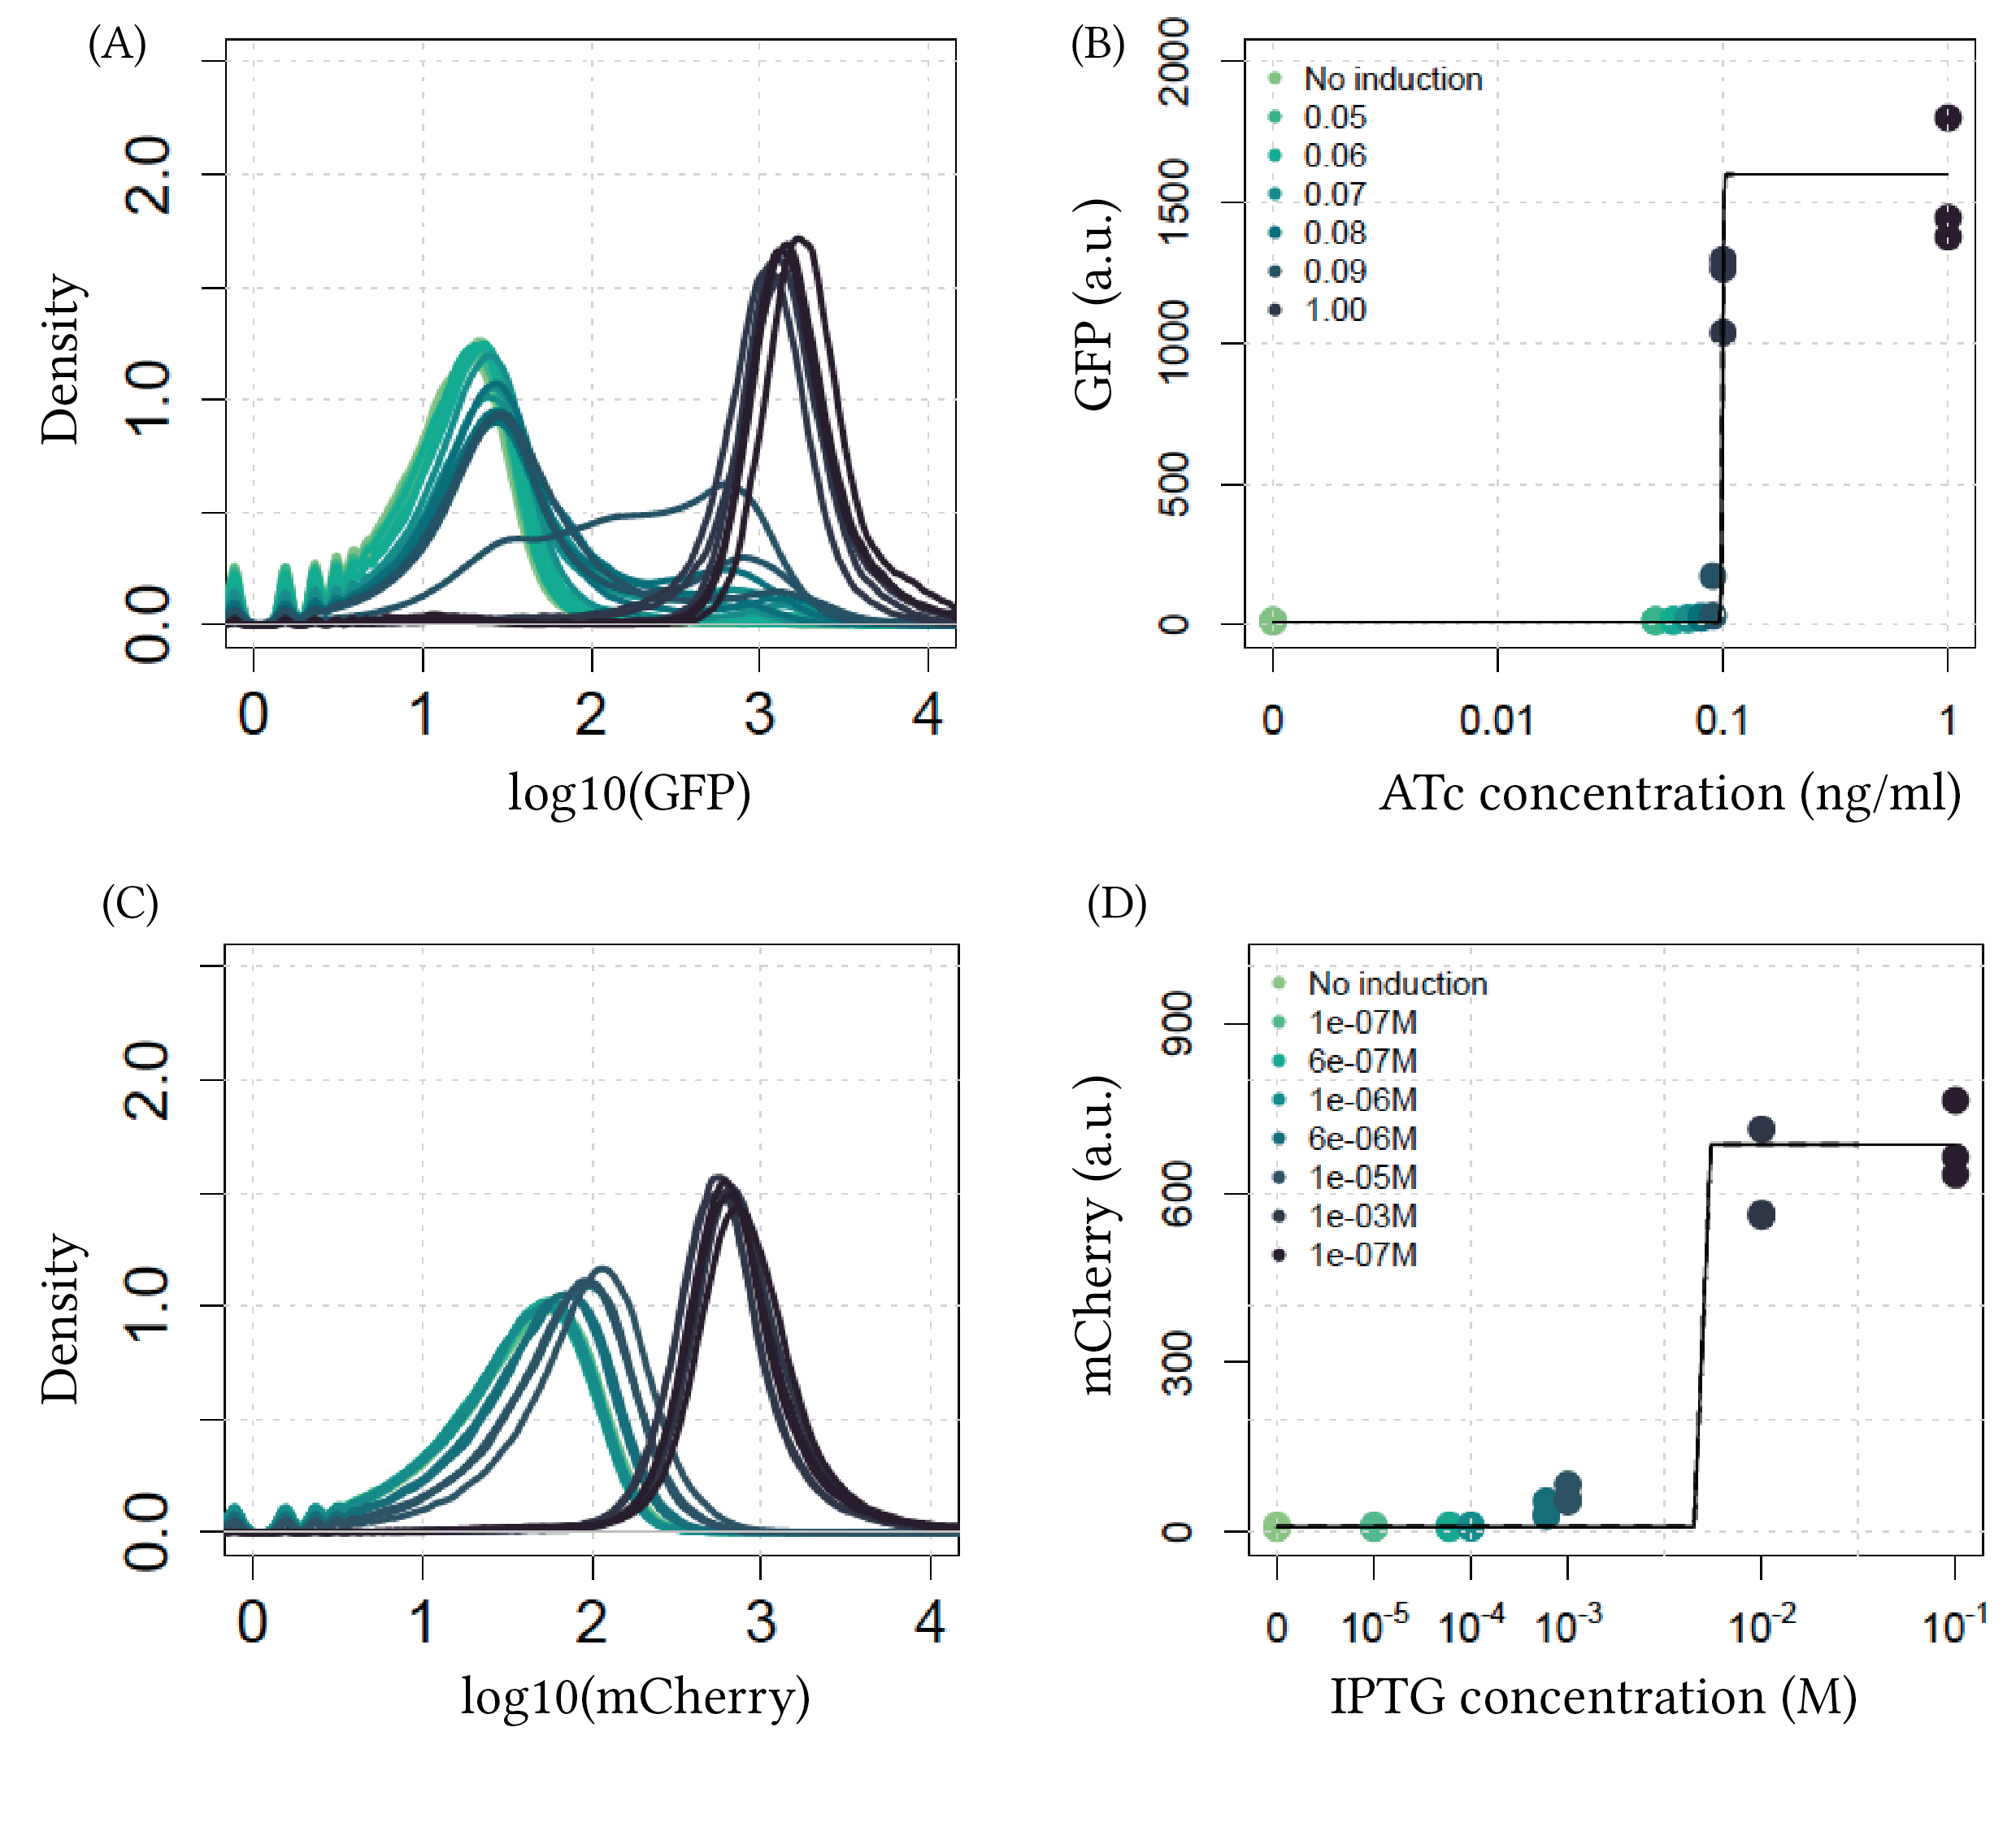
\includegraphics[width=\textwidth]{chapterCharacterisation/images/pKDL071_concentrations_model_fit.png}
\caption[LoF caption]{\label{fig:switch_concentrations_model}: (A, B) \acrshort{atc} induction of pKDL071. (C, D) \acrshort{iptg} induction of pKDL071.}
\end{center}
\end{figure*}


For the case of the \acrshort{atc} induction we observe a sharp switch between the GFP low to the GFP high state, as can be seen in the characterisation curve in Figure~\ref{fig:switch_concentrations_model}B. This is a clear indication of the bistability of this switch.

\clearpage





\section{Toggle switch time course assay}

I further analysed the pKDL071 toggle switch by investigating the time it takes for it to switch from one high state to the other. To do that I used the method outlined in Section~\ref{sec:flo_time}. I obtained separate time courses for the \acrshort{iptg} and \acrshort{atc} inductions. 

As can be seen in Figure~\ref{fig:switch_timecourse_atc} pKDL071 \acrshort{atc}  induction begins switching 1 hour after induction. Complete induction is seen at 6 hours. During the \acrshort{iptg} induction (Figure~\ref{fig:switch_timecourse_iptg}) we see a bimodal distribution at 4 hours, and induction is complete at 6 hours. We observe that during \acrshort{atc} induction there is an increase in \acrshort{gfp} fluorescence and a decrease in mCherry fluorescence, in the case of \acrshort{iptg} induction the increase in mCherry fluorescence is not as prominent. A decrease in GFP fluorescence is observed during \acrshort{iptg} induction. 

\begin{figure*}[tb]
	\begin{center}
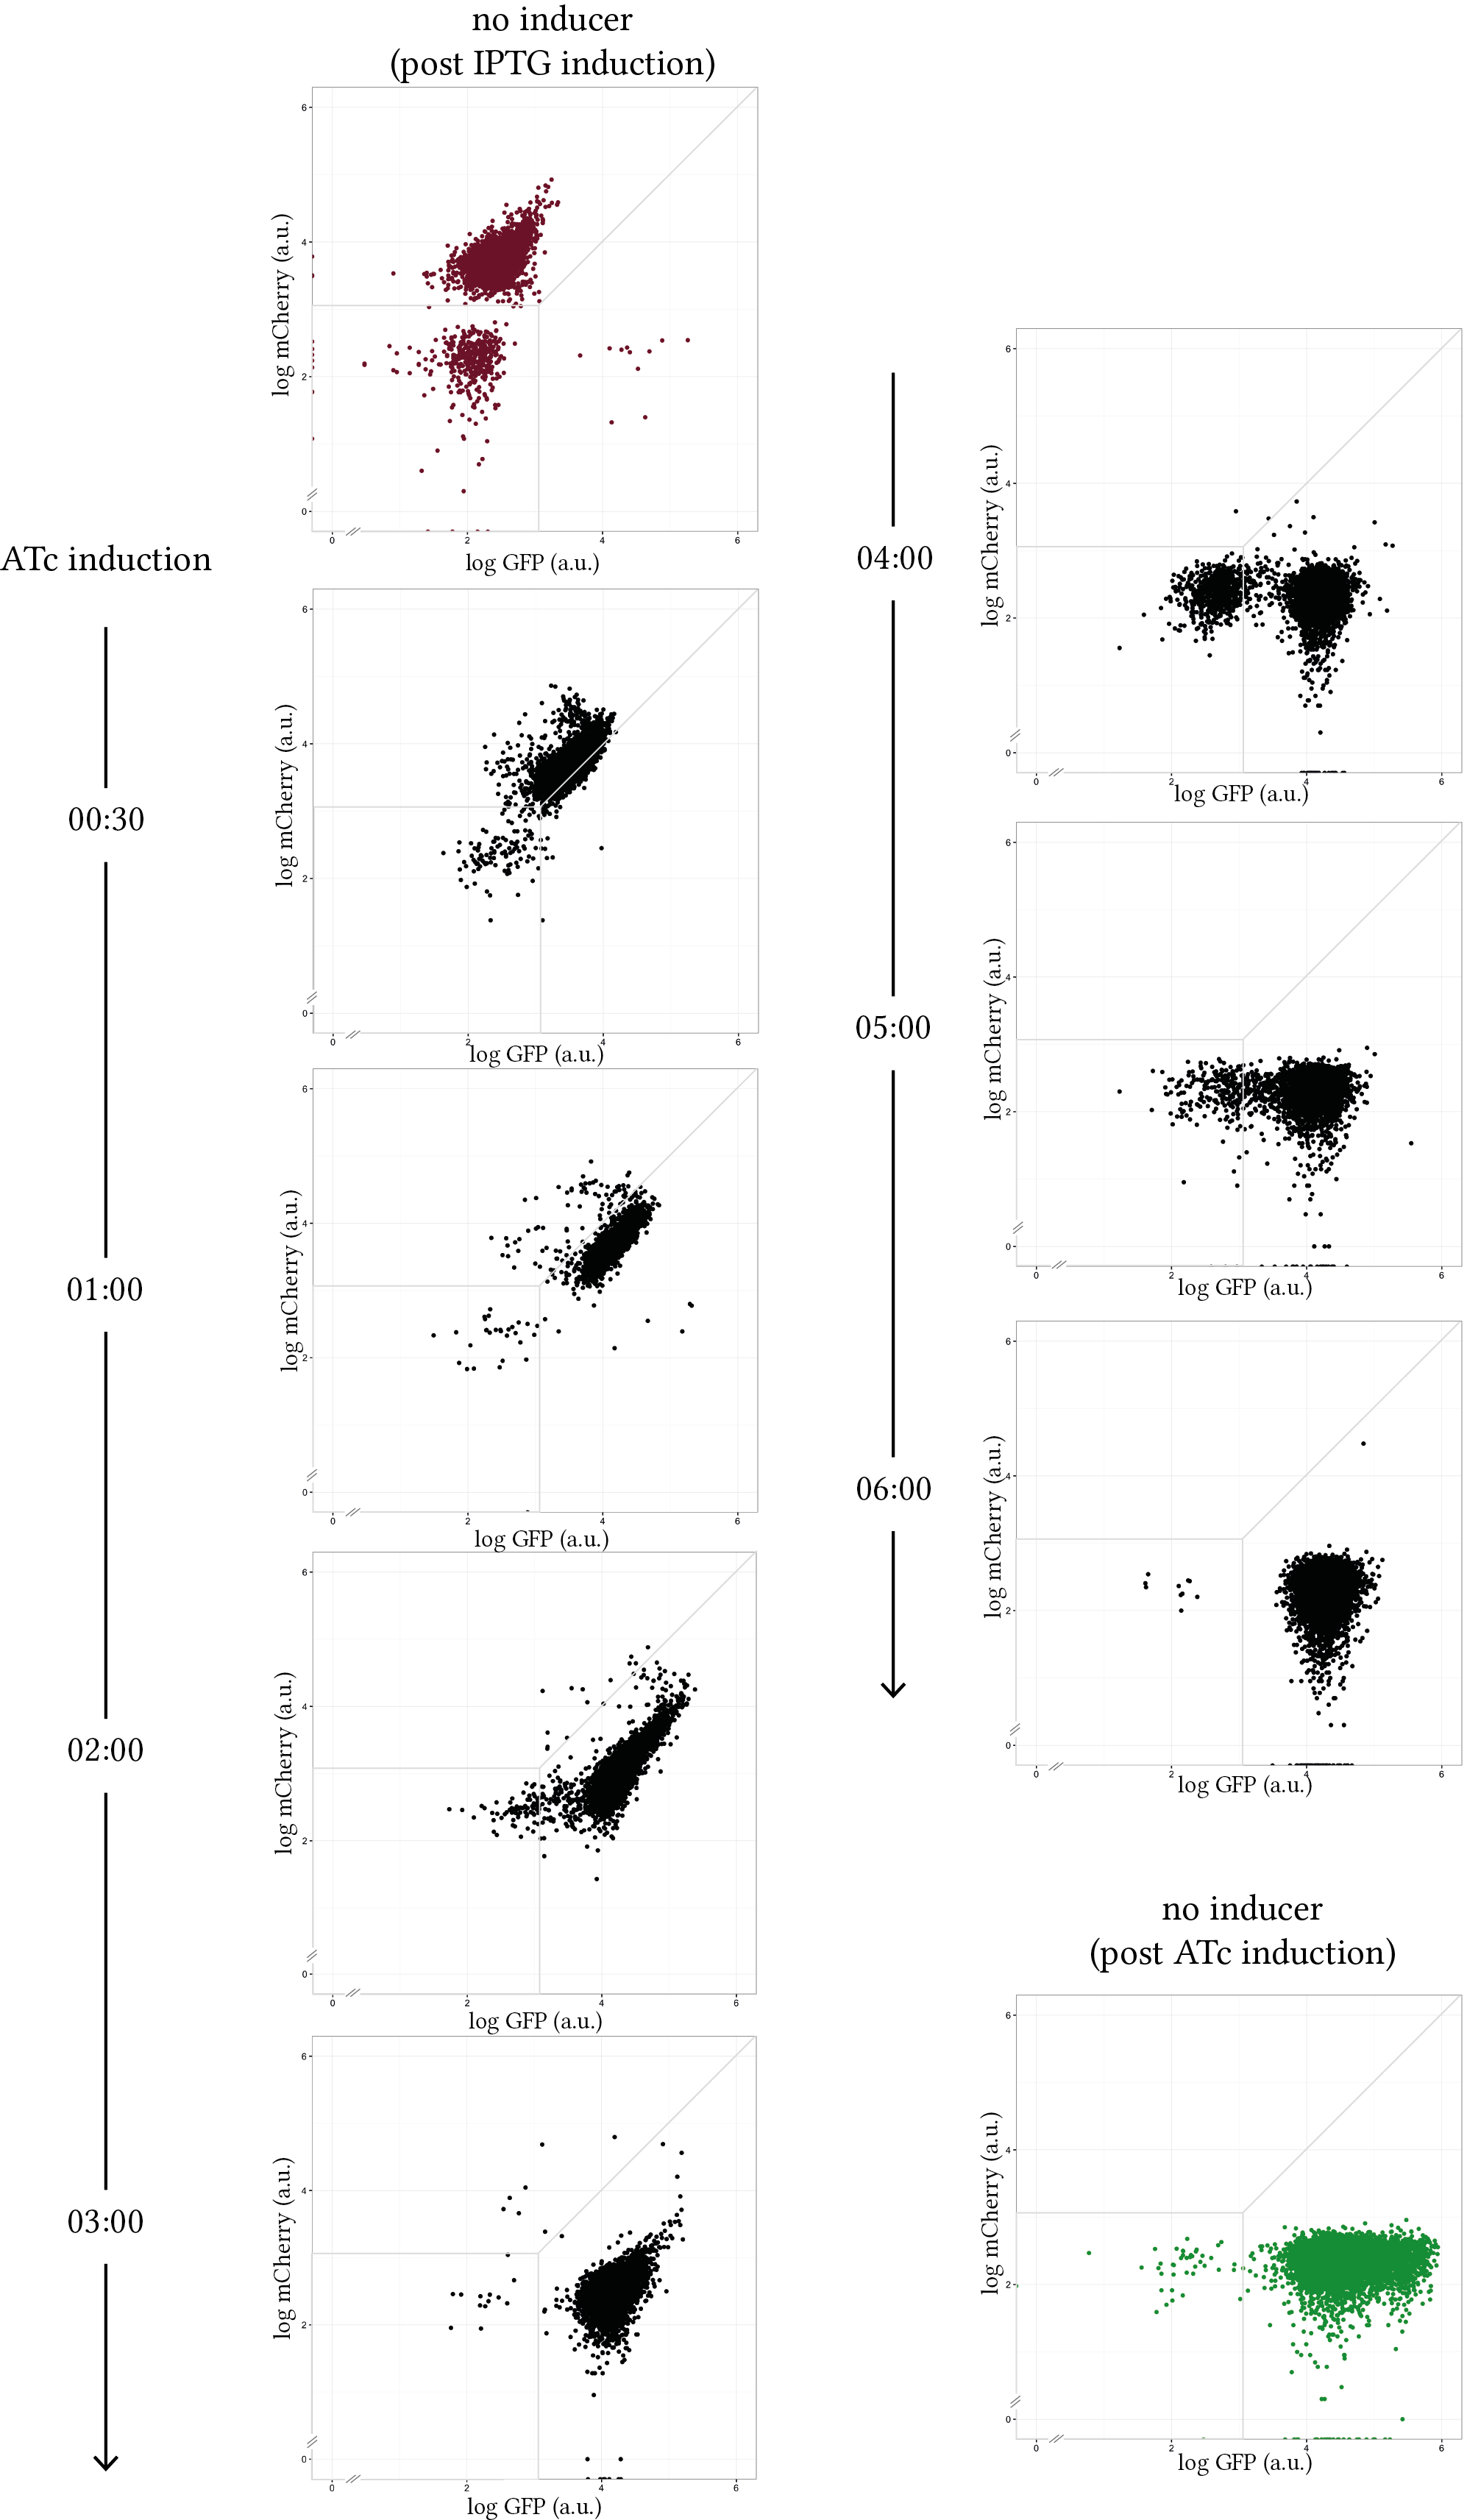
\includegraphics[scale=0.7]{chapterCharacterisation/images/pKDL071_atc_time.png}
\caption[LoF caption]{\label{fig:switch_timecourse_atc}: \acrshort{atc} induction of pKDL071 over time}
\end{center}
\end{figure*}


\begin{figure*}[tb]
	\begin{center}
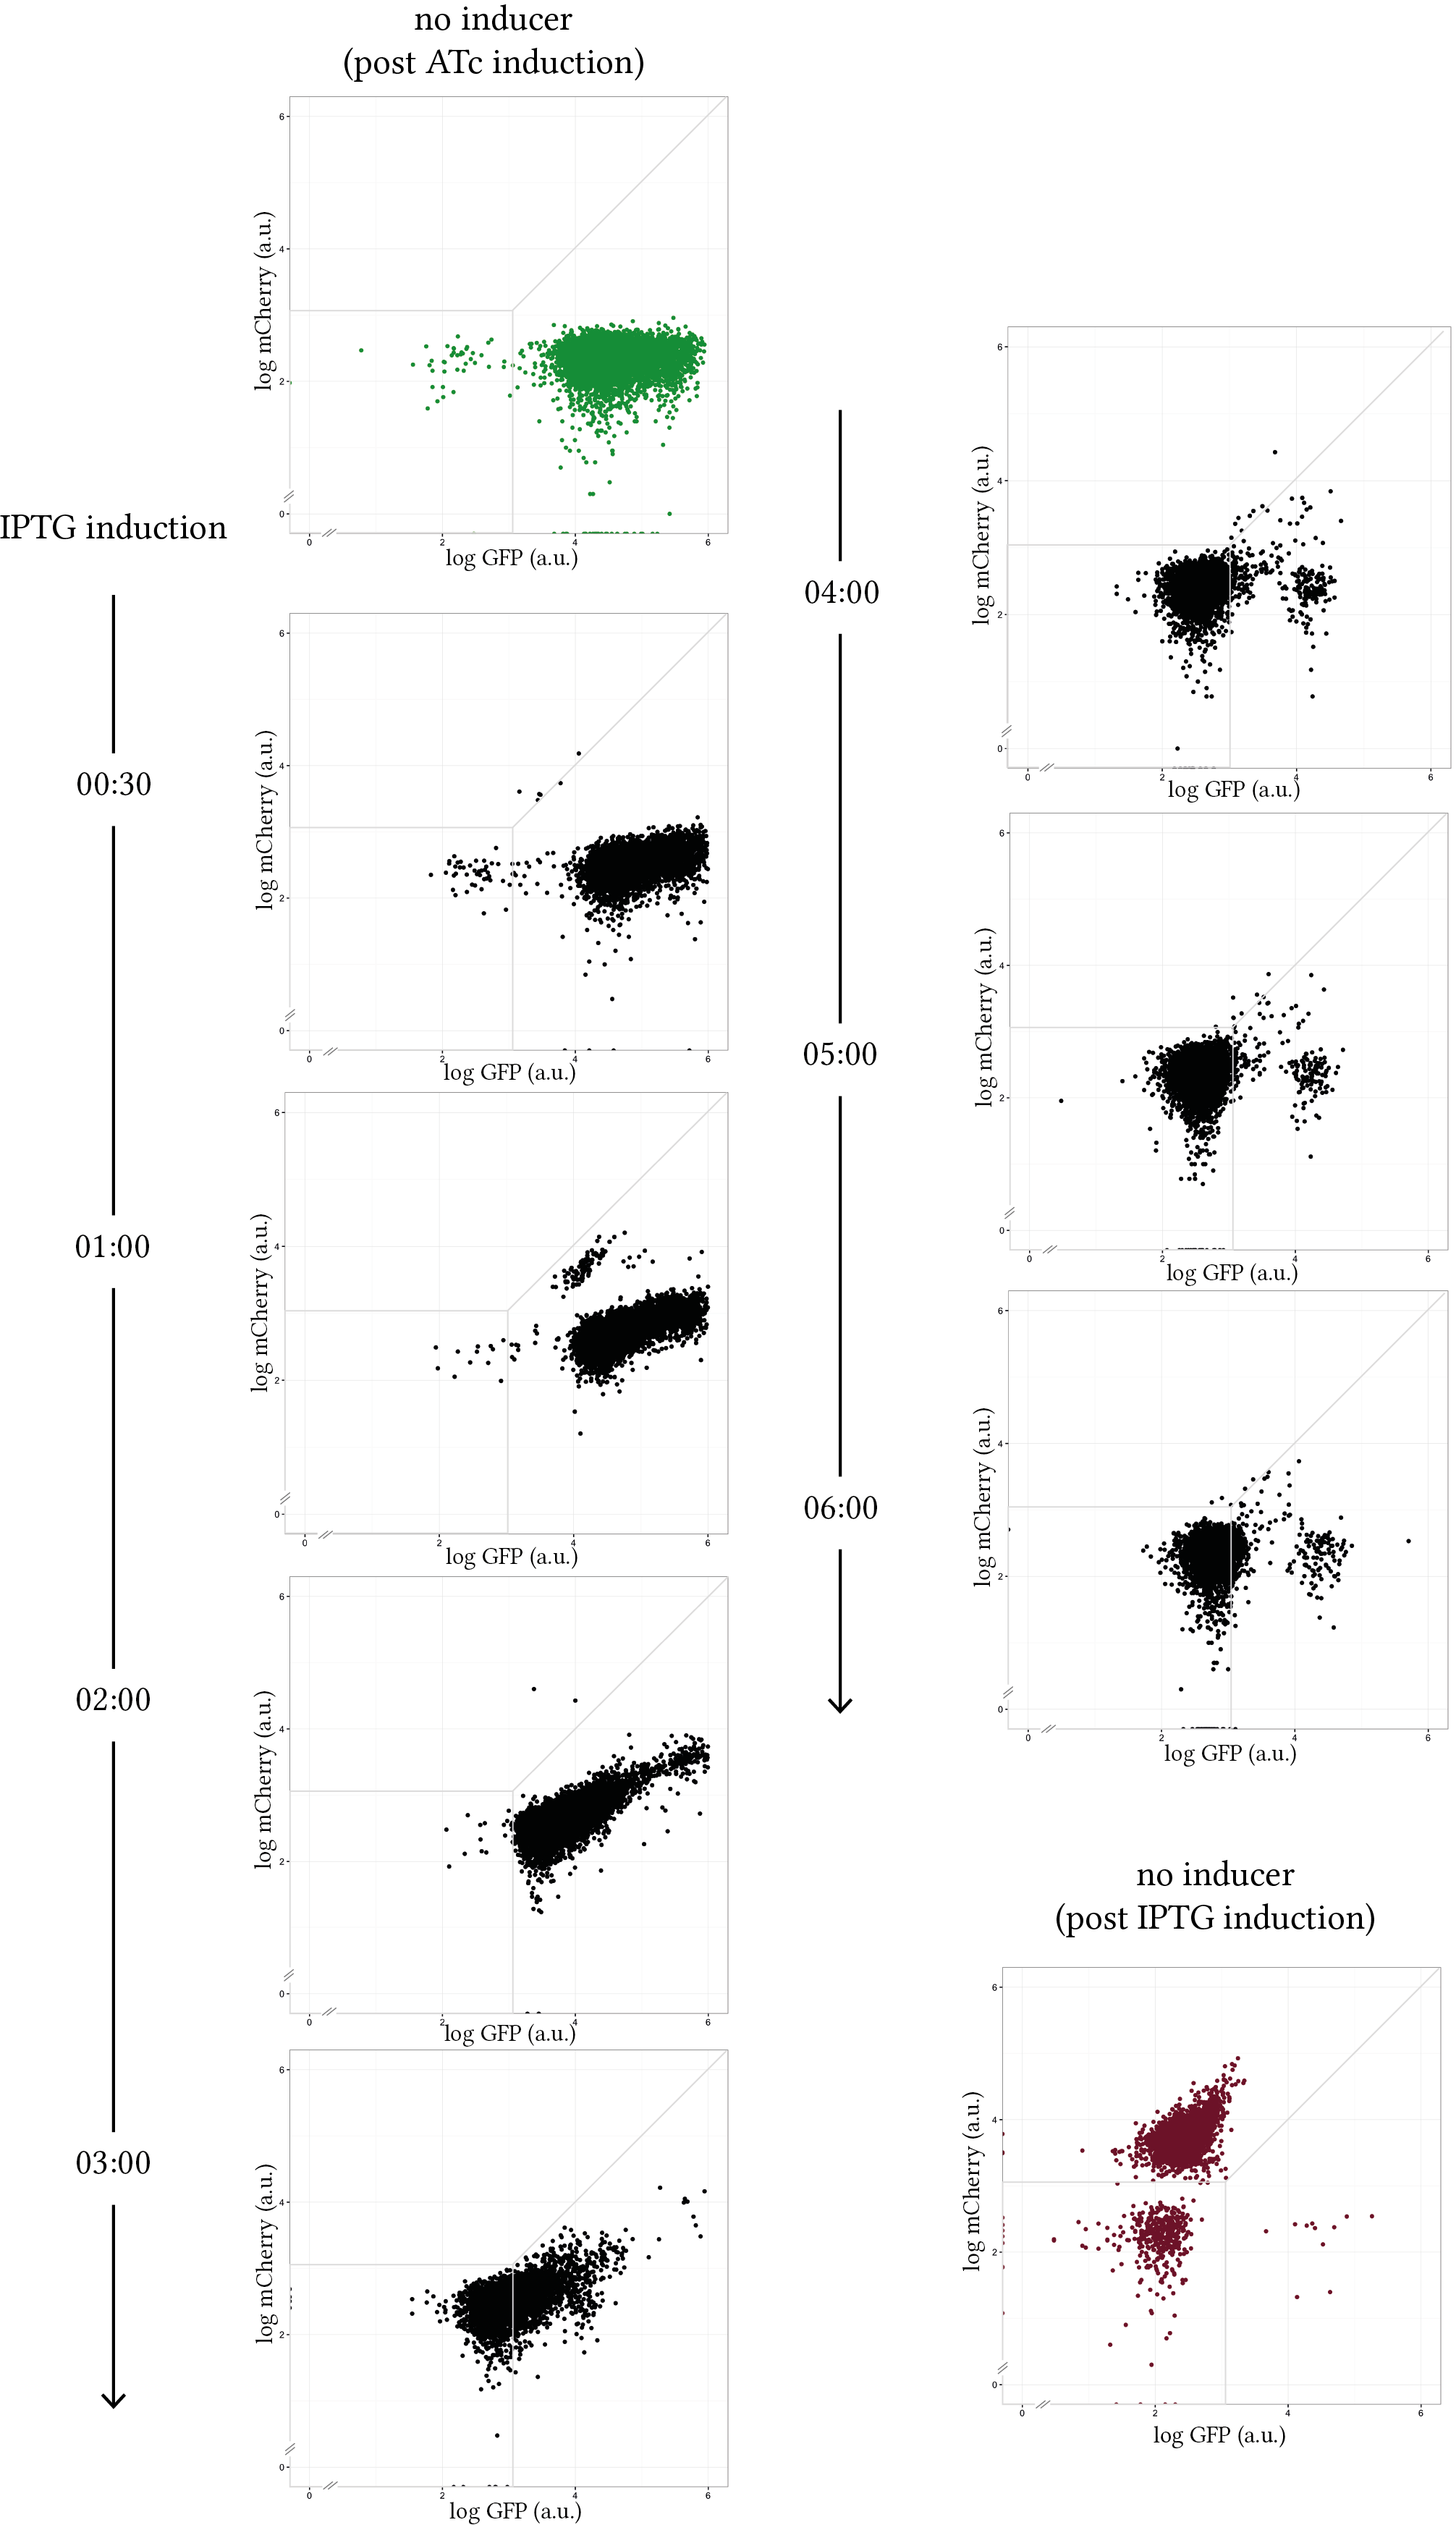
\includegraphics[scale=0.7]{chapterCharacterisation/images/pKDL071_iptg_time.png}
\caption[LoF caption]{\label{fig:switch_timecourse_iptg}: \acrshort{iptg} induction of pKDL071 over time}
\end{center}
\end{figure*}
\clearpage


%\begin{figure*}[tb]
%	\begin{center}
%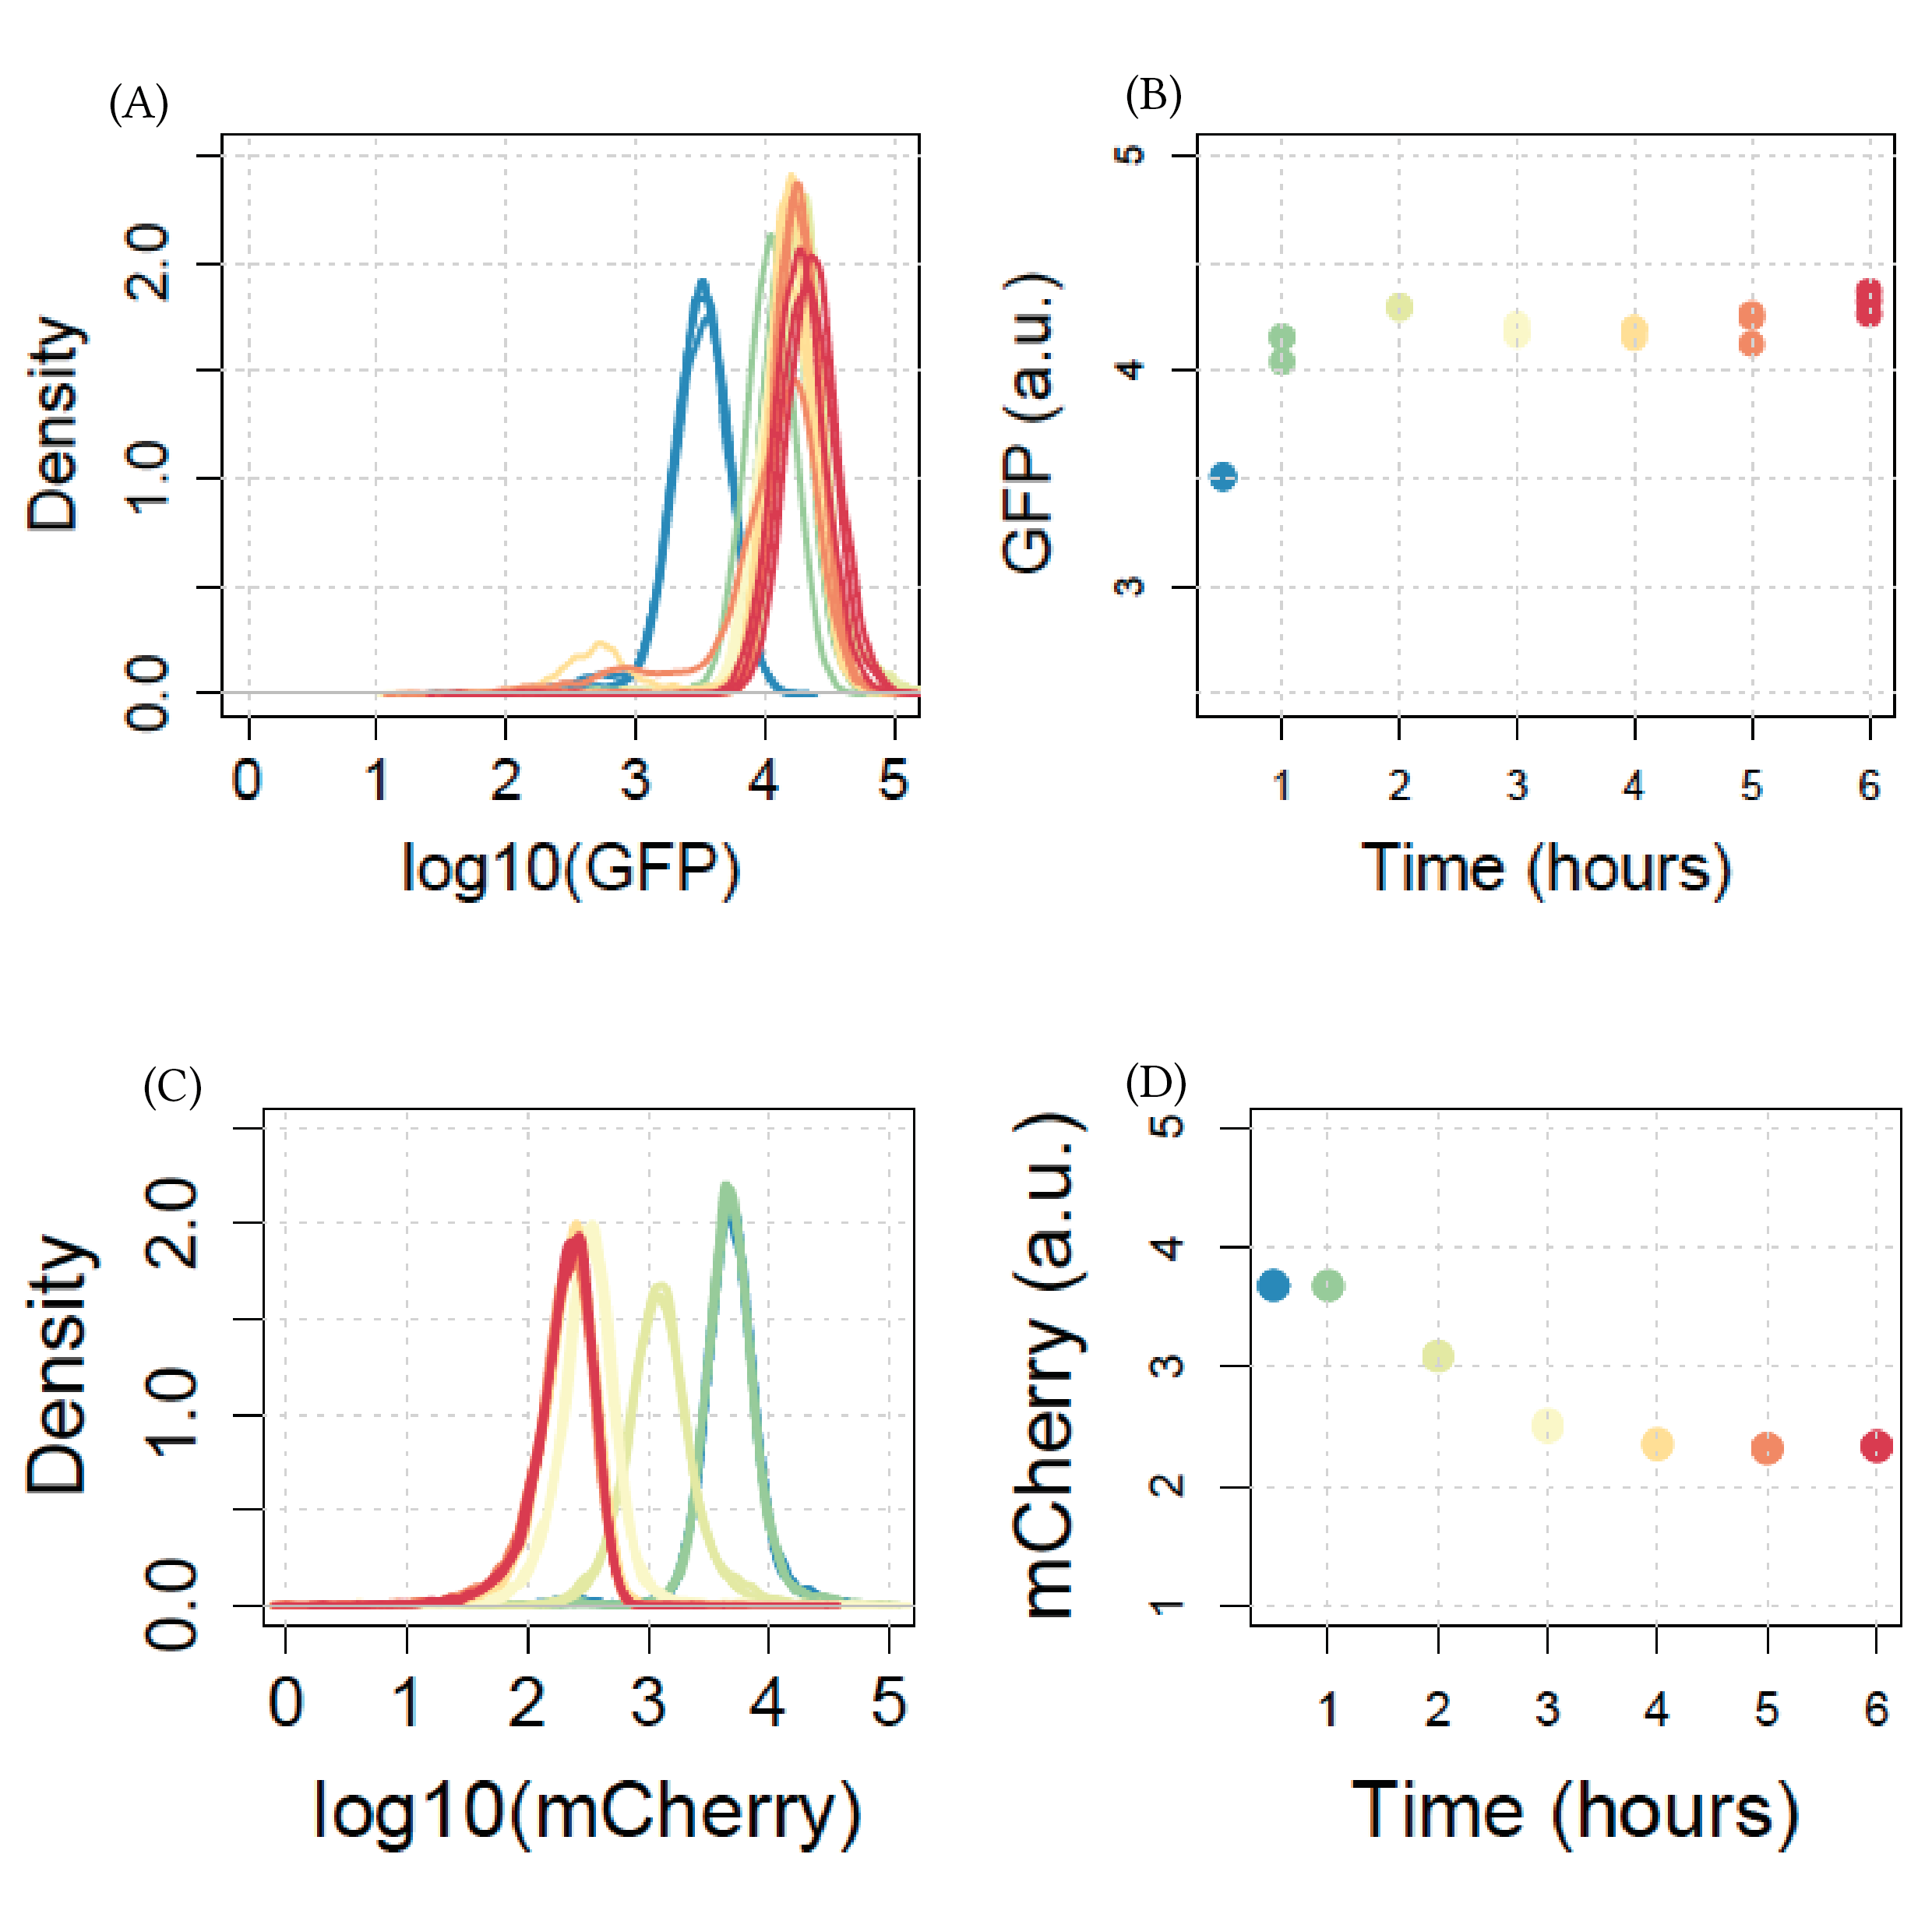
\includegraphics[scale=0.5]{chapterCharacterisation/images/atc_timecourse.png}
%\caption[LoF caption]{\label{fig:atc_timecourse}: \acrshort{atc} induction of pKDL071 over time}
%\end{center}
%\end{figure*}
%
%\begin{figure*}[tb]
%	\begin{center}
%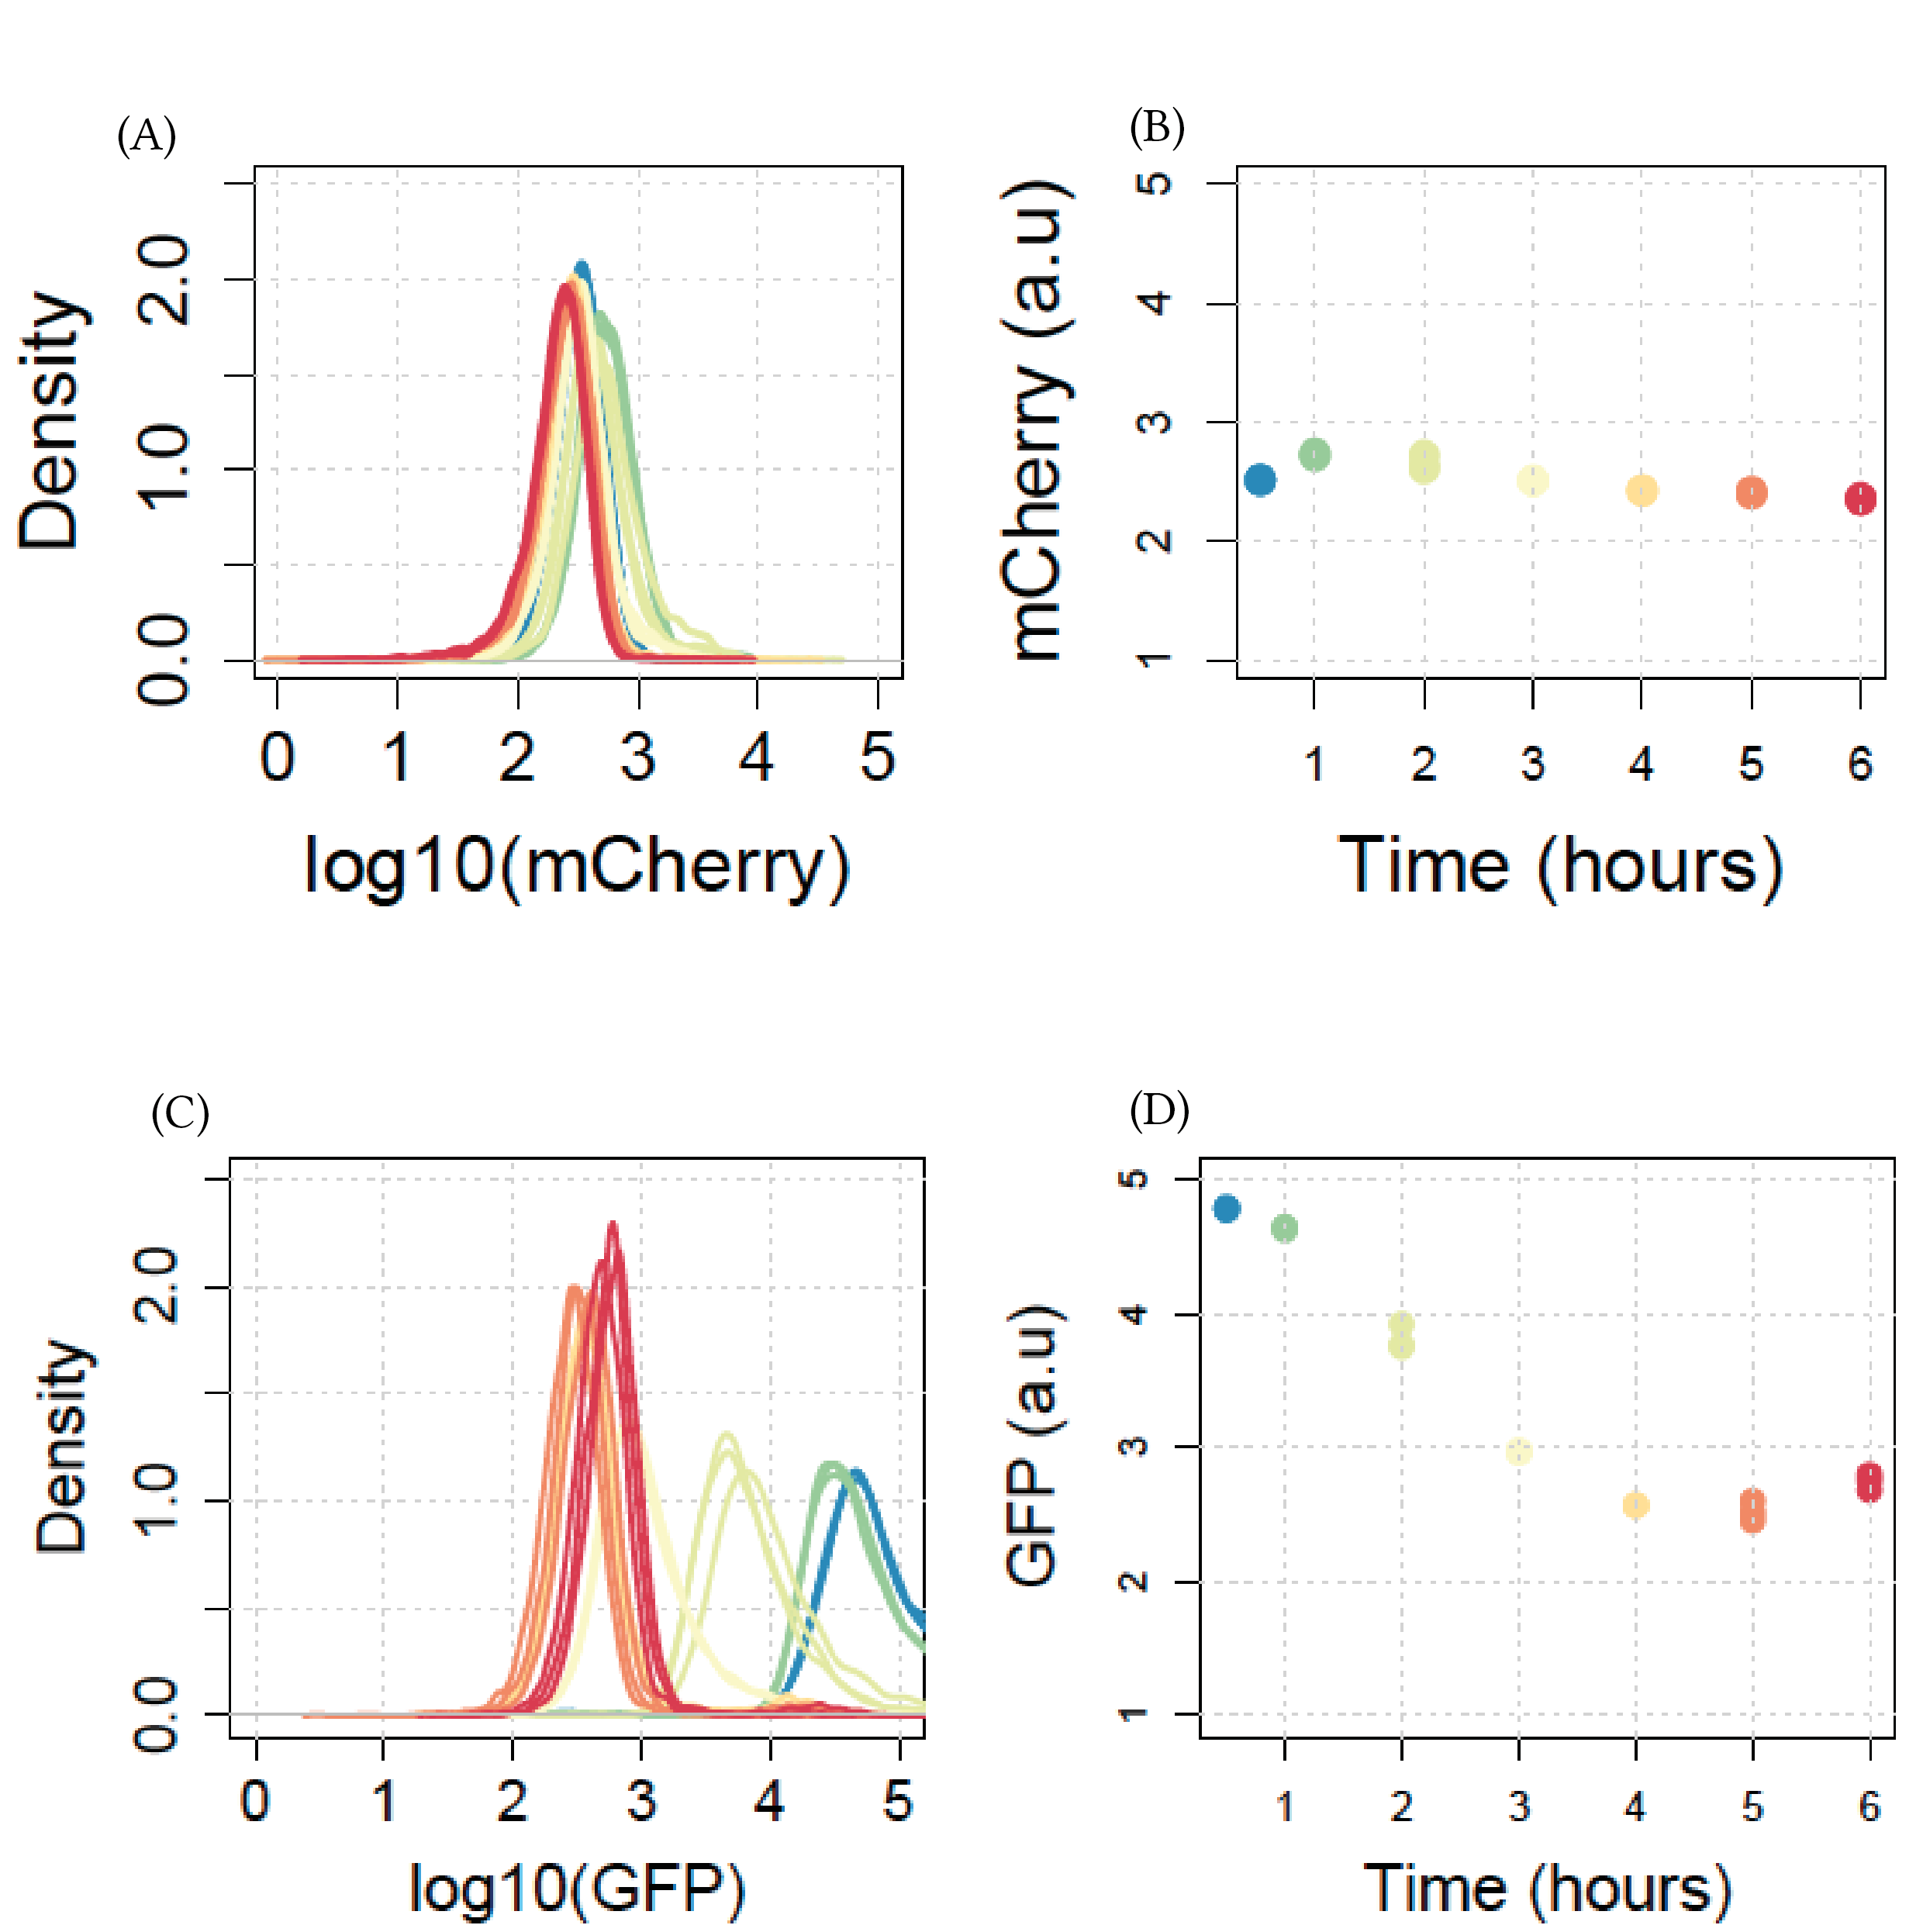
\includegraphics[scale=0.5]{chapterCharacterisation/images/iptg_timcourse.png}
%\caption[LoF caption]{\label{fig:iptg_timecourse}: \acrshort{iptg} induction of pKDL071 over time}
%\end{center}
%\end{figure*}
%\clearpage

\section{Discussion}

Here I characterised the genetic toggle switch experimentally. First I study the effect of the two inducers \acrshort{atc} and \acrshort{iptg} on the growth rate of the selected chassis \textit{E. coli} K-12 MG1655. I find that there is no detrimental effect to the bacterium by the inducers. I also find that which state the switch is on has no effect on the growth rate of the bacteria. In order for this toggle switch to be used in a synthetic biology application, it is important that both sides of the switch have an equivalent burden onto the chassis. If one of the steady states creates a larger burden and slows down the growth of the bacteria, this can create an imbalance in the population. If the toggle switch-bearing bacterial population exists in an environment with competing bacteria, for example the gut microbiome, and one of the two states creates a larger burden, this would cause the switch-bearing population to become less competitive compared to the non switch-bearing population. It is therefore crucial that the state of the switch does not affect the competitiveness of the chassis.  


I further characterised the switch by determining the minimum inducer concentration necessary to change the state of the switch. I find that for \acrshort{atc} induction, a minimum of \SI{0.09}{\nano\gram\per\milli\liter} is required to cause the switch to go to a GFP high state. For \acrshort{iptg} induction I find that a minimum of \SI{0.001}{M} is required to flip the switch to an mCherry high state. This information is critical for using this switch in other applications. Both sides of the switch are very sensitive to inducer concentrations, as the concentrations required to observe a change in fluorescence are very small. 

Furthermore I find that this toggle switch, pKDL071, is faster to respond to a change in \acrshort{atc} concentration that to a change in \acrshort{iptg} concentration. For \acrshort{iptg} induction we observe a change in fluorescence after 3-4 hours of induction. For \acrshort{atc} induction we can see a difference within an hour of induction. This result is in agreement with~\textcite{Litcofsky:2012gr}. This difference in response times must be taken into account when using the pKDL071 switch for other applications. This difference could be due to maturation times of the fluorescent proteins. \textcite{Macdonald:2012el} found that mCherry half-maturation time is 150 mins, whereas the GFP variant used here, GFPmut3b has been especially mutated for fast action~\autocite{Cormack:1996gv}. ~\textcite{Cormack:1996gv} found that whereas wild type GFP is detectable 1-2 hours after induction, GFPmut3b is detectable 8 minutes after induction. This difference could account for the different response times observed here, but further investigation is required. 

\section{Summary}


In this chapter I summarised the experiments carried out for the analysis of the genetic toggle switch. I used the pKDL071 plasmid and characterised its switching behaviour over various inducer concentrations and over time. I found the concentration of each inducer necessary to flip the switch as well as the time it takes for the change to be observed. Furthermore, I investigated the effect of the inducers on the growth rate of the chassis and found that they have no effect. In the next chapter I use the data collected in the chapter to fit to the more realistic toggle switch models used in Chapter (XXX). 




